% !TeX encoding = UTF-8
\documentclass[twoside,english,1p,final,sort&compress]{elsarticle}
\usepackage[T1]{fontenc}
\usepackage[utf8]{inputenc}
\pagestyle{headings}
\usepackage{amsthm}
\usepackage{gensymb}
\usepackage{xspace}
\usepackage{amsmath}
\usepackage{accents}
\usepackage{multirow}
\usepackage{arydshln}
\usepackage{xcolor}
\usepackage{amssymb}
\usepackage{subcaption}
\usepackage{adjustbox}
\usepackage{placeins}
\usepackage{ulem}
\usepackage[colorlinks = true]{hyperref}

% To have Times only in text not maths
\renewcommand{\rmdefault}{ptm}

\makeatletter

\theoremstyle{plain}
\newtheorem{thm}{\protect\theoremname}

% specify here the journal
\journal{International Journal of Mechanical Sciences}

% use this if you need line numbers
\usepackage{lineno}

\makeatother

\usepackage{babel}
\providecommand{\theoremname}{Theorem}

\DeclareRobustCommand{\w}{\mbox{\large\ensuremath{\mathsf{w}}}}
\DeclareRobustCommand{\dotp}{\boldsymbol{\cdot}}
\DeclareRobustCommand{\e}[1]{{\rm e}^{#1}}
\DeclareRobustCommand{\lay}[1]{^{(#1)}}
\DeclareRobustCommand{\mdot}[1]{\accentset{\mbox{\bfseries .}}{#1}}
\DeclareRobustCommand{\ie}{\emph{i.e.}\@\xspace}
\DeclareRobustCommand{\eal}{et \emph{al.}\@\xspace}
\DeclareRobustCommand{\eg}{e.g.,\@\xspace}
\DeclareRobustCommand{\RMSE}{\text{E}_\text{RMS}}
\DeclareRobustCommand{\AARE}{\text{E}_\text{AAR}}
\DeclareRobustCommand{\R}{\text{R}}
\DeclareRobustCommand{\ps}{\text{s}^{-1}}
\DeclareRobustCommand{\mr}[2]{\multirow{#1}{*}{#2}}
\DeclareRobustCommand{\MPa}{\text{MPa}}

% This is used to add comments into the text
%
% Will have to be removed from final version
%
\usepackage{soul}
\usepackage{color}
\definecolor{VWyellow}{RGB}{255,251,150}
\DeclareRobustCommand{\OP}[1]{\begingroup\sethlcolor{VWyellow}\textcolor{red}{\hl{\textbf{O.P.:} #1}}\endgroup}
\DeclareRobustCommand{\OPP}[1]{\begingroup\sethlcolor{VWyellow}\textcolor{red}{\hl{\textbf{O.P.:} In previous sentence #1}}\endgroup}

\begin{document}
\begin{frontmatter}

\title{Interpolation and extrapolation based performance measurement of Analytical and Artificial Neural Network models in predicting hot deformation behavior of a medium carbon steel}

\author[LGP]{Pierre Tize Mha}
\author[ETS]{Prashant Dhondapure}
\author[LGP]{Amèvi Tongne}
\author[ETS]{Mohammad Jahazi}
\author[LGP]{Olivier Pantalé\corref{cor1}}
\ead{Olivier.Pantale@enit.fr}
\ead[url]{http://www.enit.fr}

\cortext[cor1]{Corresponding author}

\address[LGP]{Laboratoire Génie de Production, INP/ENIT, Université de Toulouse, 47 Av d'Azereix, Tarbes, 65016, France}
\address[ETS]{École de Technologie Supérieure, 1100 Rue Notre Dame O, Montréal, QC H3C 1K3, Canada}

\begin{abstract}
In the present work, a critical analysis of the most commonly used analytical models and of recently introduced Artificial Neural Network based models is conducted to evaluate their prediction accuracy within and outside the experimental interval used to generate them. To this end, the high-temperature deformation behavior of a medium carbon steel was studied over a wide range of strains ($0.0-0.7$), strain rates ($0.001~\ps-5~\ps$) and temperatures ($1050\celsius-1250\celsius$) using hot compression tests on a Gleeble $3800$ thermomechanical simulator. The experimental flow curves were then modeled using Johnson-Cook, Modified Zerilli-Armstrong, Hansel-Spittel, Arrhenius, the recently proposed PTM model, as well as an Artificial Neural Network model with $3$ inputs, $2$ hidden layers of $15$ and $7$ neurons, respectively, and 1 output. The Mean Absolute Relative Error (MARE) and the Root Mean Square Error (RMSE) values were used to quantify the predictive accuracy of the analyzed models. The results indicated that the Johnson-Cook and Modified Zerilli-Armstrong models presented significant error, MARRE of  $21.20\%$, while the Hansel-Spittel, PTM and Arrhenius models could predict the behavior of this alloy with an error of about $3.56\%$ error. The Artificial Neural Network model, on the other hand, showed excellent agreement, with less than a $0.62\%$ error, between the predicted and experimental flow curves. To further validate the performance of the above models, their ability to interpolate and extrapolate the experimental data was also tested. The Hansel-Spittel, PTM and Arrhenius analytical models showed a good interpolation and extrapolation capability with the notable superiority of the Arrhenius model over the other two. The Artificial Neural Networks model was however, still the most performant among all the models. A correlation factor was proposed to extend the applicability of some of the investigated models to deformation conditions not included in the original experimental plan.
\end{abstract}

\begin{keyword}
Johnson-Cook \sep Zerilli-Armstrong \sep Arrhenius \sep Hansel-Spittel \sep Artificial Neural Network  \sep interpolation  \sep extrapolation 
\end{keyword}

\end{frontmatter}
\linenumbers

%----------------------------------------------------------------------------------
\section{Introduction\label{sec:Introduction}}
%----------------------------------------------------------------------------------
Large size forged blocks made of medium carbon high-strength steels are extensively used in the automotive industry as dies for the production of bumpers and dashboards through the plastic injection process. The manufacturing process of the large blocks starts with ingot casting, followed by open die forging, and a quench and temper heat treatment process to achieve the desired mechanical properties  \cite{chadha2017deformation,chadha2018influence,murugesan2019two}. In recent years, in order to respond to the market demand, larger size forgings have had to be produced. In parallel, more stringent conditions related to chemical homogeneity, hardness, grain size and mechanical properties from the surface to the core of the forged block have been required. Of the three manufacturing steps (casting, forging and heat treatment), forging is where the most important microstructural changes take place, and which greatly influences the final properties that can be achieved \cite{murugesan2019hybrid,chadha2020microstructure,sripada2022effect}. The open die forging process is fundamentally a hot compression process during which work strengthening effects, such as hardening (WH) and precipitation,  take place concomitantly with softening phenomena such as   recovery and recrystallization under static and/or dynamic \cite{tian2022deformation,tavakoli2019ferrite}. It has also been reported that phase transformation can occur during deformation. The extent and intensity of the above phenomena strongly depend on three macroscopic quantities namely, the strain $\varepsilon$, the strain rate $\mdot\varepsilon$ and the temperature $T$  \cite{ ebrahimi2017flow,Ashtiani-2012,He-2013, Changizian-2012}. 
 
Considering the large size of blocks, a purely experimental approach, based on trial and error, can not be used by industry, and  therefore, reliable predictive tools, such a Finite Element analysis (FEA) codes, have been developed, and are commercially available. However, the prediction reliability of such analyses is a function of the accuracy of the material constitutive model, which describes the mutual interactions between the strain, the strain rate, and the temperature during deformation. As mentioned above, precipitation and phase changes are considered negligible as deformation takes place in the austenite at temperatures above the dissolution temperature of most carbides. Hence, most constitutive models depend on macroscopic parameters which influence the hardening and softening of the material. A large number of phenomenological, semi-empirical, or physical models \cite{Rusinek-2010, Shin-2010, Lin-2011, Pantale-2021} have been developed. Among these, the Johnson-Cook (JC) \cite{Johnson-1983}, Hansel-Spittel (HS) \cite{chadha2018approach}, and Zerilli-Armstrong (ZA) \cite{Zerilli-1987} models are the best known and most widely available in FEA codes. Despite their simplicity, each of them suffers from certain shortcomings: as reported by Jia \eal \cite{Jia-2021}, the JC model suffers from a lack of non-coupling between the strain, the strain rate and the temperature,  while the HS model is better adapted for higher strain rate deformation conditions \cite{chadha2018approach}. To circumvent these shortcomings, several modified model forms have been developed \cite{chadha2018approach, Rule-1998, Vural-2003, Lin-2010, Lin-2012}. However, as reported by many authors \cite{Li-2013, Zhang-2015, Zhou-2019}, even after adjusting the constants, the high temperature flow behavior, particularly when dynamic recrystallization takes place, can not be accurately predicted and none of the models is able to accurately predict the flow behavior outside the experimental testing interval that was used to determine the model constants. Due to its more physics-based formulation, the ZA model and its modified form, MZA, \cite{NematNasser-2004, Lennon-2004, Muralli-2017, Cheng-2021, Muralli-2021}, and the Arrhenius-type hyperbolic sine constitutive models are preferred to the JC and HS  models both for the prediction of the hot deformation behavior and microstructure analysis of the material \cite{Jonas-1969, Mostafaei-2012, Zhang-2012}. The Arrhenius formulation has been revised to achieve a more accurate determination of the activation energy for high temperature deformation \cite{Slooff-2007, Lin-2008-C}. To overcome the strong dependency of the models on specific alloy types, Tize Mha \eal \cite{TizeMha-2022} recently proposed a constitutive model, PTM, whose formulation is independent of the alloy type. This formulation is based on the MZA model and the polynomial functions of undefined order that are used during the identification. However, in the PTM model, the high order of the polynomial function (up to $10$ in some cases) can affect its accuracy. 

The Artificial Neural Network (ANN) is an approach used to predict the flow stress behavior of materials without requiring a mathematical formulation of the flow law. It is therefore not necessary to postulate a mathematical expression to identify the parameters of the model. Since the behavior of materials is highly nonlinear at high temperatures, and depends on many factors which are also nonlinear, the evaluation of the flow stress behavior by an analytical model whose parameters are identified by a classical regression method is limited. Faced with these limitations, ANN models are of major interest because they are particularly suited to deal with complex and nonlinear relationships. Consequently, ANNs have been successfully applied to predict the flow stress behavior of materials under hot working conditions \cite{Lin-2008-ANN, Lu-2011-ANN, Ashtiani-2016-CSP, Stoffel-2019-NNB}. Although ANN models can predict well the material flow behavior, there is a problem with its implementation in finite element software, as reported by Pantalé \eal \cite{Pantale-2021}. In fact, the implementation of a constitutive model in an FEA code requires the derivatives of the model with respect to strain, strain rate and temperature.

Although progress has been made in improving constitutive models to better predict the flow stress behavior of materials, problem still persist with the model's efficiency. Indeed, a model is considered appropriate for predicting the material's behavior if its predictions and experimental results correlate well. It is questionable whether a model that correctly describes the behavior of a material in a defined experimental window can be used to accurately predict its behavior for conditions different from those for which it was identified. In other words, the question is whether interpolation and extrapolation techniques can be used to extend the applicability of a constitutive equation for different materials and processing windows.

The present work aims to address the preceding question using a combination of the recently introduced PTM model and ANN. To this end, initially, hot compression tests, simulating the open die forging process, are carried out and the flow curves  generated are modeled using the above--mentioned constitutive equations and an ANN model developed in this work. Then, the interpolation and extrapolation capabilities of each model are evaluated and a solution proposed, responding to the main question of the paper. The results are validated based on experimental work carried out here in and on data obtained from the literature. 



%----------------------------------------------------------------------------------
\section{Materials and Experiments\label{sec:Materials}}
%----------------------------------------------------------------------------------

%----------------------------------------------------------------------------------
\subsection{Experimental procedure}
%----------------------------------------------------------------------------------

The material used in this study consists of a medium carbon steel whose chemical composition is given in Table \ref{tab:Composition}.
\begin{table}[h!]
\centering
\caption{Chemical composition of medium carbon steel, Fe = balance.}
\begin{tabular}{lccccccc}
	\hline
	Element &  C   &  Mn  &  Mo  &  Si  &  Ni  &  Cr  &  Cu  \\ \hline
	Wt~\%   & 0.30 & 0.89 & 0.52 & 0.34 & 0.68 & 1.86 & 0.17 \\ \hline
\end{tabular}
\label{tab:Composition}
\end{table}
Cylindrical samples were machined with an initial diameter of $d=10$~mm and a height of $h_0=15$~mm.
Hot compression tests were performed on a Gleeble-3800 thermomechanical simulator (see Figure \ref{fig:Gleeble3800}), for $5$ temperature levels, namely, $1050\celsius$, $1100\celsius$, $1150\celsius$, $1200\celsius$ and $1250\celsius$ with the $6$ strain rates of $0.001~\ps$, $0.01~\ps$, $0.1~\ps$, $1~\ps$, $2.0~\ps$ and $5~\ps$.
\begin{figure}[!ht]
\centering
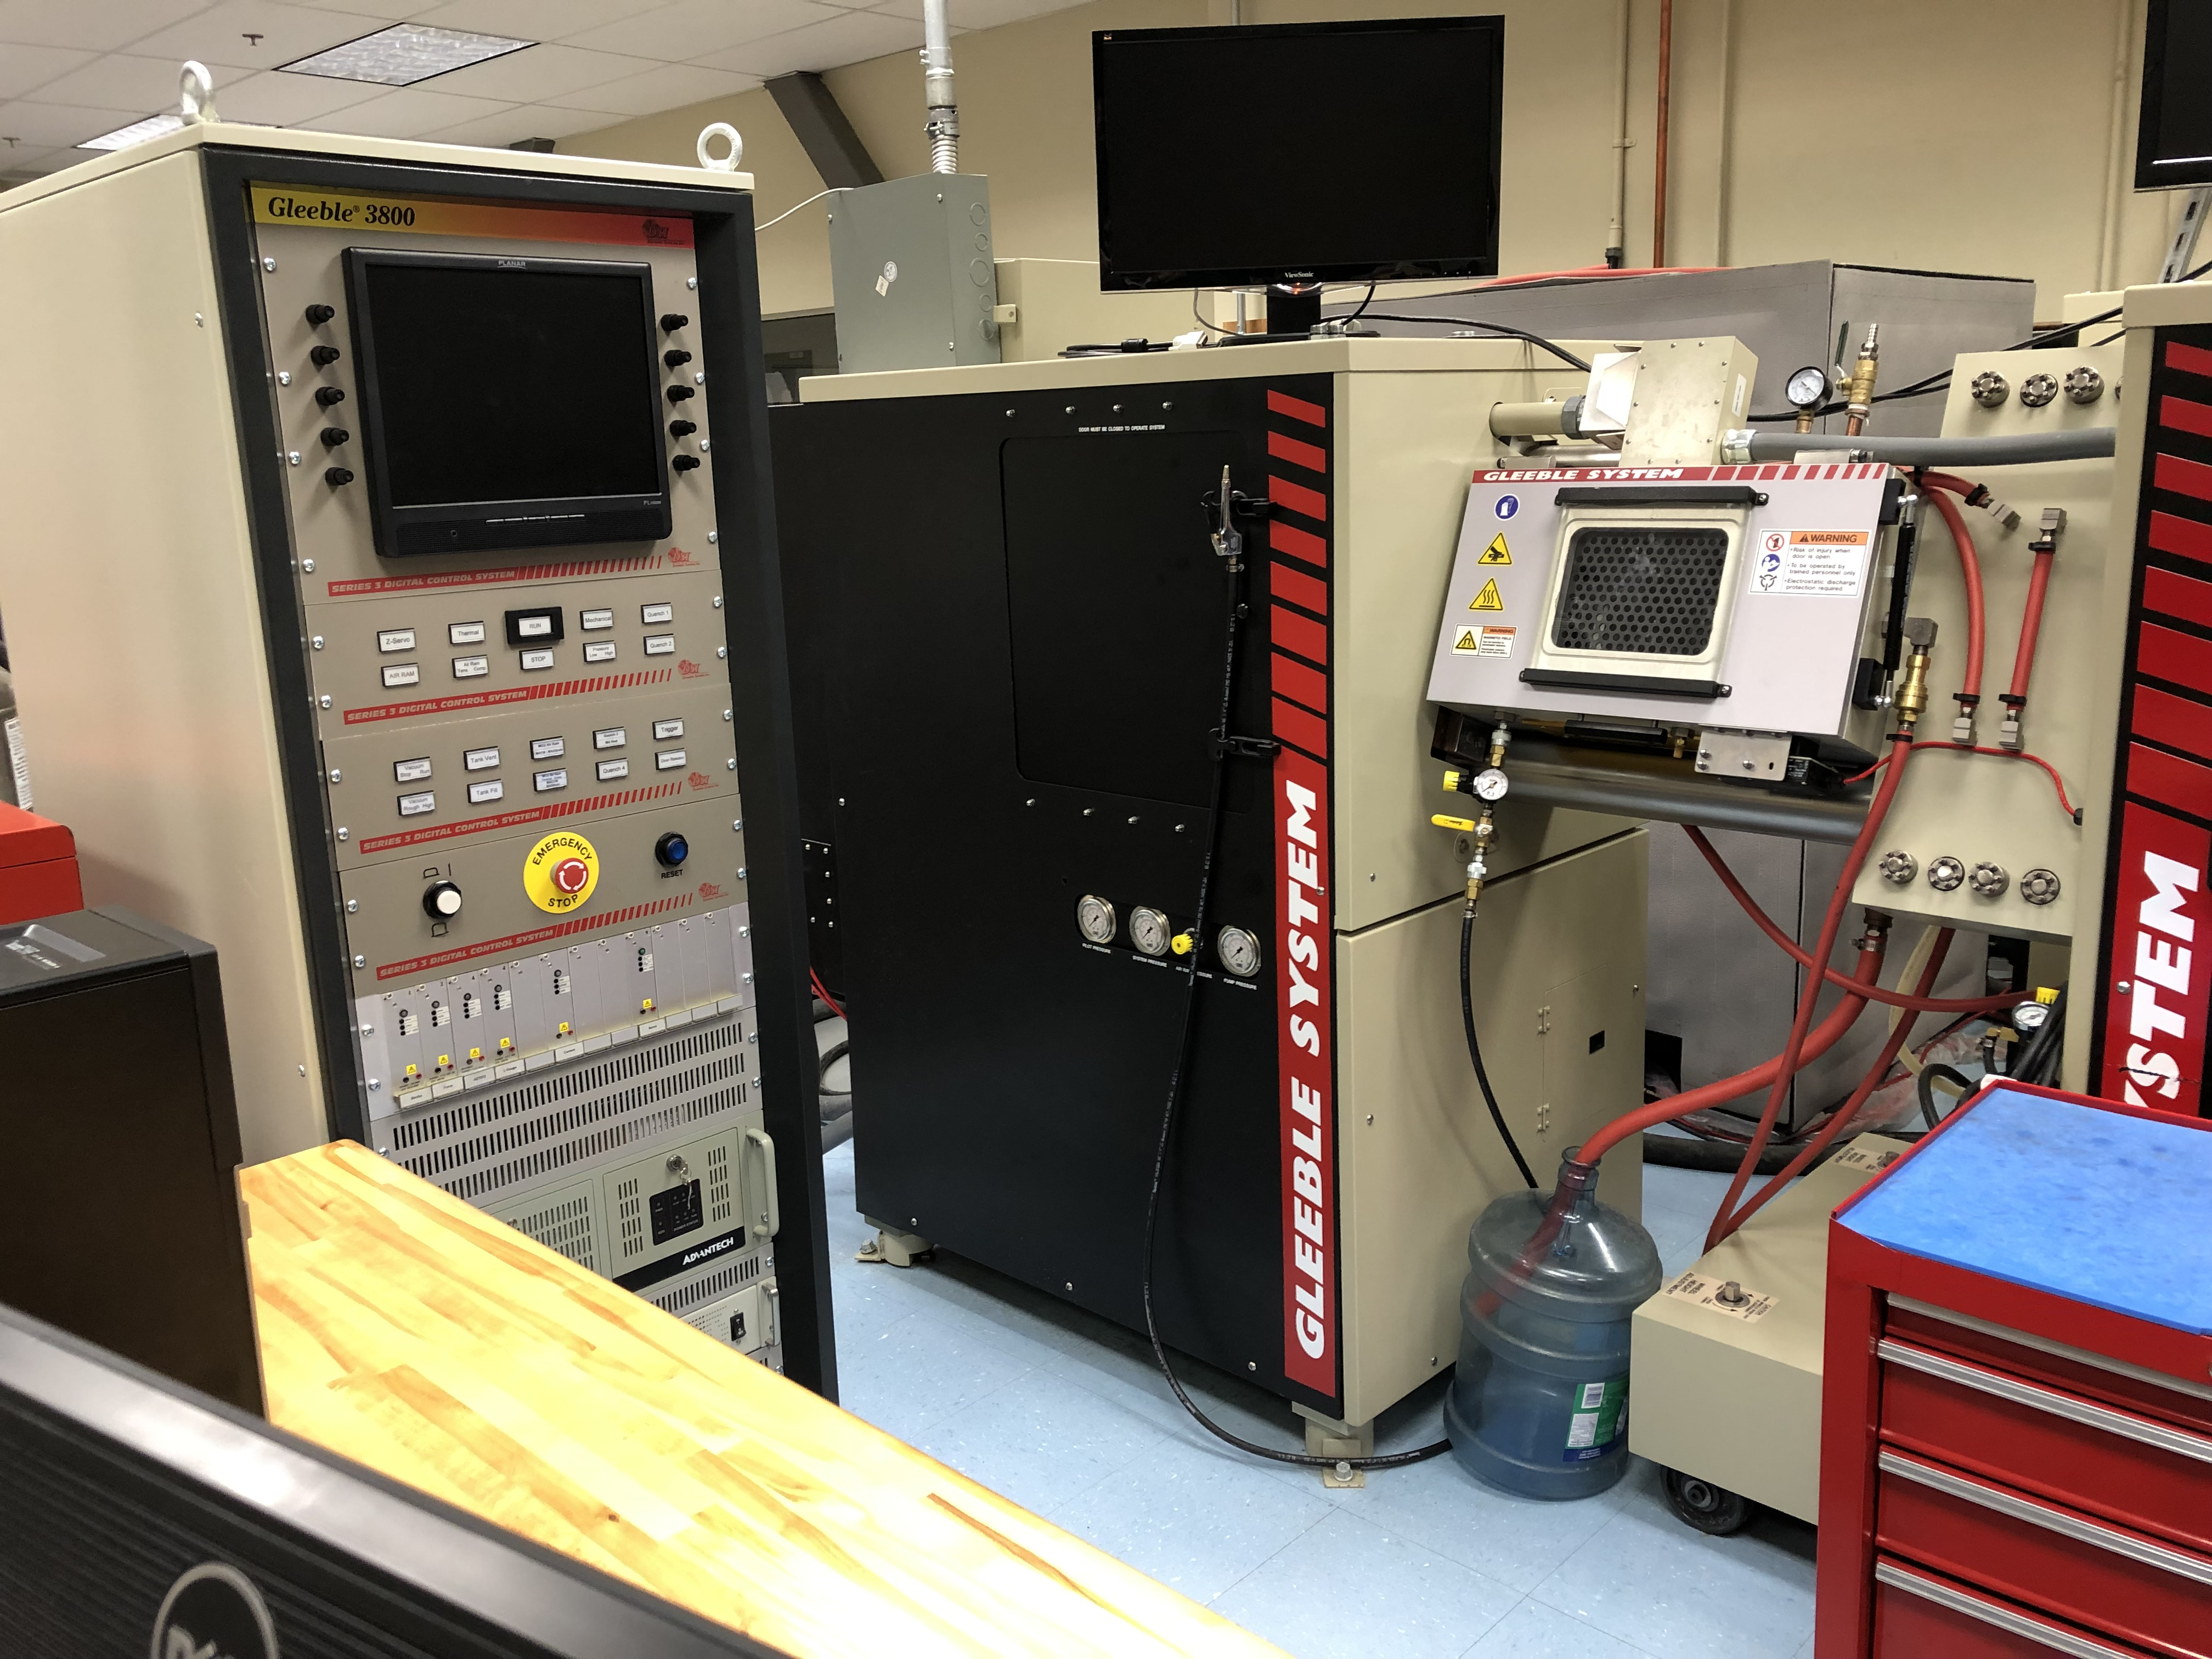
\includegraphics[width=0.7\columnwidth]{Figures/Gleeble-3800}
\caption{The Gleeble-3800 thermomechanical simulator system used for this study}
\label{fig:Gleeble3800}
\end{figure}
Thin tantalum sheets were used as lubricating material at the contact surface of the anvils and samples to minimize friction during testing. As shown in Figure \ref{fig:GleebleProcess}, the samples were heated to a temperature of $1260\celsius$ with a heating rate of $2$\celsius/s and held at this temperature for $5$~min to eliminate thermal gradients. They were then cooled down with a rate of $1$\celsius/s to the test temperature and then held at constant temperature for $1$~min before deformation. During the compression phase, the temperature of the specimen is kept constant by the thermal control system of the machine. After compression, the specimen is quickly quenched to freeze its microstructure for later analysis. Figure \ref{fig:GleebleProcess} also shows the aspects of the specimens before and after the compression test: $h_0$ and $r_0$ are the height and radius before compression and $h$, $r_m$ and $r_t$ are the height, large radius and small radius of the specimen after compression, respectively.
\begin{figure}[!ht]
\centering
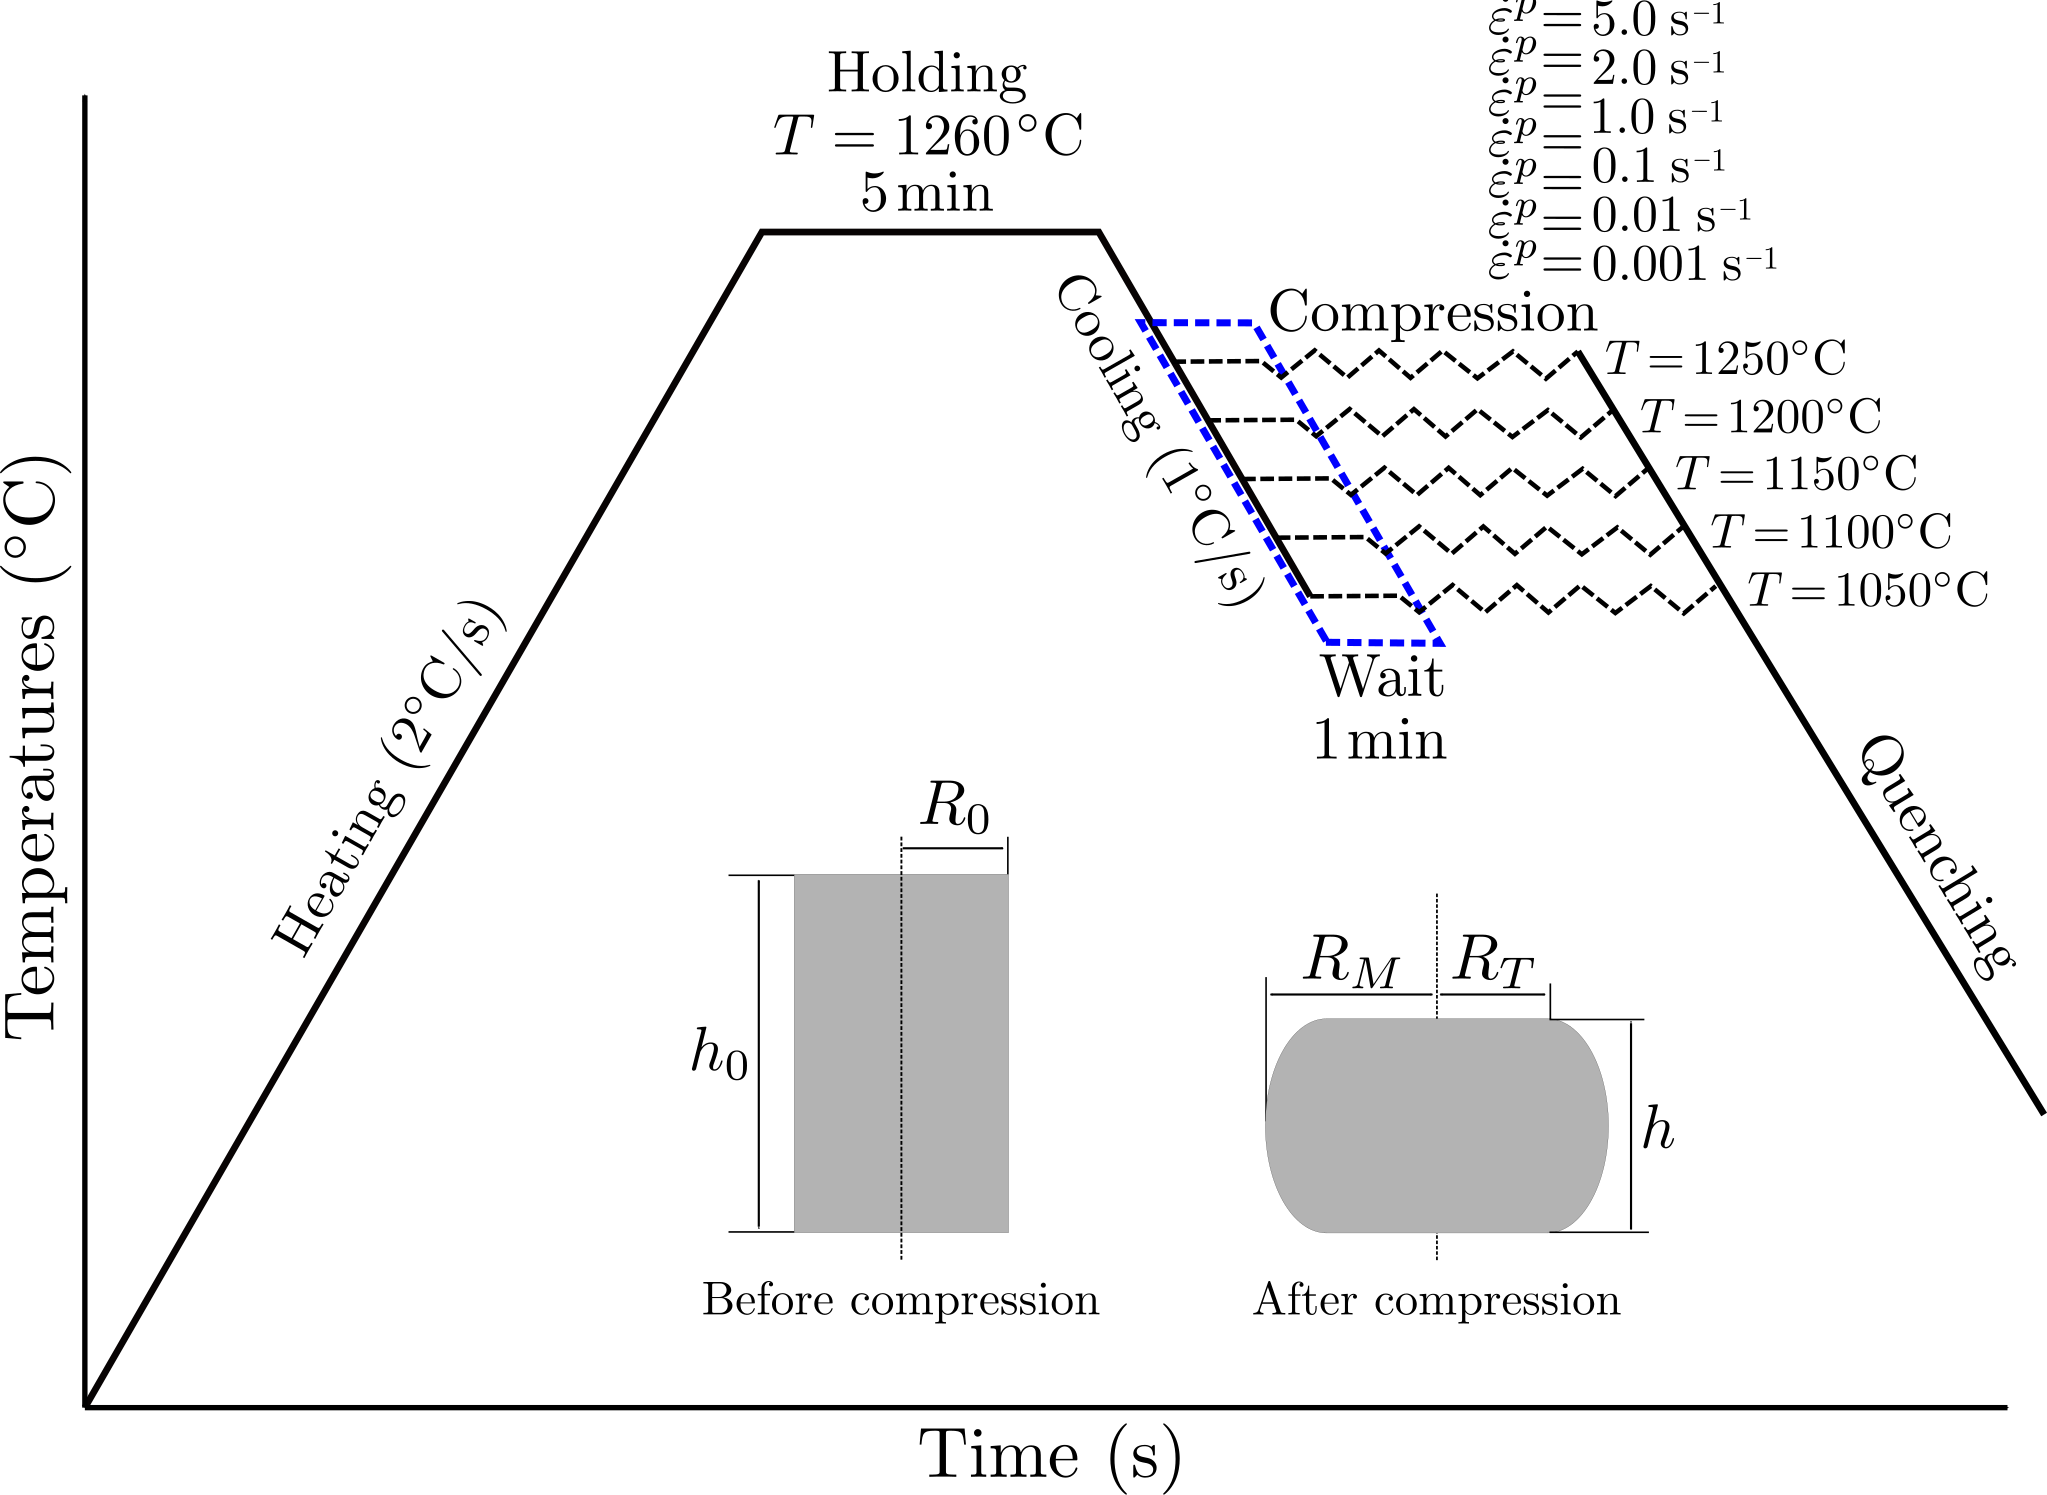
\includegraphics[width=0.8\columnwidth]{Figures/GleebleProcess}
\caption{Schematic diagram of the experimental process.}
\label{fig:GleebleProcess}
\end{figure}

The stress-strain curves are automatically exported from the Gleeble thermomechanical simulator system as the true stress and true strain according to the L-gauge, where the formula to get the curves is given by $\sigma=F/A$ and $\varepsilon=\ln\left(h_0+\Delta h / h_0\right)$ or C-gauge,  having the following formulas: $\sigma = 4F/\pi(d+\Delta d)^2$ and $\varepsilon = 2\ln(d/(d+\Delta d))$ with $d = 2r_0$, and where $F$ is the force as measured by the Gleeble load cell. As raw data contains noises, savgol$\_$filter method from the scipy library is used to remove noise and provide smoother data. To allow further use of the data in numerical simulations, elastic parts are removed.

%----------------------------------------------------------------------------------
\subsection{Compression tests results\label{sec:ComTestResults}}
%----------------------------------------------------------------------------------

The set of flow stress $\sigma^y$ versus strain $\varepsilon$ curves obtained from compression tests performed on the Gleeble-3800 simulator for each test condition (6 strain rates and 5 temperatures) is presented in Figure \ref{fig:RawData}.
\begin{figure}[!ht]
\centering
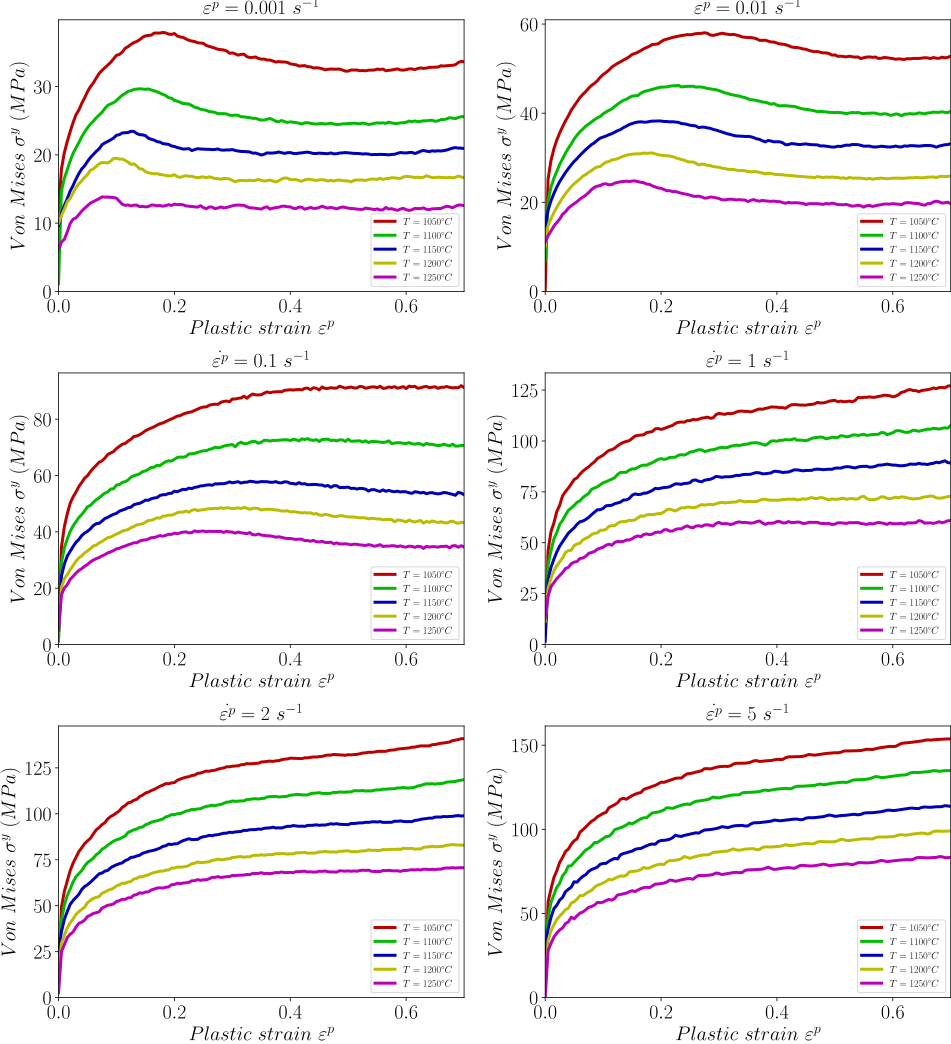
\includegraphics[width=\columnwidth]{Figures/rawData}
\caption{Stress-strain curves of medium carbon alloy extracted from the Gleeble device at various temperatures $T$ and strain rates $\mdot\varepsilon$.}
\label{fig:RawData}
\end{figure}
All data curves contain $700$ equidistant strain values up-to $\varepsilon=0.7$.
Therefore, there are $6$ strain rates and $5$ temperatures, and the database consists of $21~000$ data points.
The overall behavior of these curves shows that the flow stress $\sigma^y$ increases with increasing strain rate $\mdot\varepsilon$ but decreases with increasing temperature $T$.
It should be noted that the strain also influences the flow stress.
Indeed, for the lowest strain rates $\mdot\varepsilon$, the flow stress $\sigma^y$ increases with the strain $\varepsilon$ until a value of about $\varepsilon=0.2$ to $0.3$, and then decreases to maintain a more or less constant value until the end of the test.
For the highest strain rates ($1~\ps$, $2~\ps$, and $5~\ps$), the flow stress increases throughout the test.
The slight increase in stress at low strain rates, when the strain is large, has been reported to be due to friction between the sample and the anvil during the test \cite{buckley2001deformation}. The frictional effect is also visible when testing at low strain rates, as the effect of lubrication decreases over time, and friction thus increases. The increase of stress observed at the beginning of the deformation and up to $0.1$ is due to work hardening (WH). After $0.1$ and up to $0.2$, the flow stress shows a continuous reduction with increasing stress until a peak or an inflection of the work-hardening rate. This behavior indicates that thermal softening becomes more and more predominant until it exceeds WH. At this step, the stress curve shows three different patterns with the increasing strain: (i) gradual decrease to a steady state with DRV/DRX softening. This is the case for all deformation temperatures and strain rates between $0.001$ and $0.1$ \text{s}$^{-1}$, except for those at $1050^\circ$C and $1100^\circ$C; (ii) higher stress levels without significant softening and work-hardening at $1050^\circ$C and $1100^\circ$C and a $0.1$ $\text{s}^{-1}$  strain rate ; and (iii) continuous increase with significant work hardening (all deformation temperatures and strain rate of $1$ \text{s}$^{-1}$). Therefore, it can be concluded that the softening due to DRX, characterized by a flow curve with a single peak followed by a steady-state flow, takes place at high temperatures and low strain rates. In contrast, at higher strain rates and lower temperatures, the higher work hardening rate slows down the rate of softening due to DRX, and therefore, both the peak stress and the onset of steady-state flow are shifted to higher strain levels. In fact, the drop observed in
stress is because of DRX occurrence at all temperatures and strain rates of $0.001$–$5$ $\text{s}^{-1}$. As an example, Figure \ref{fig:Micrography} shows the medium carbon microstructure held for $5$~min at $1260\celsius$ before and after the compression phase.
\begin{figure}[!ht]
\centering
\begin{subfigure}[b]{0.45\columnwidth}
\centering
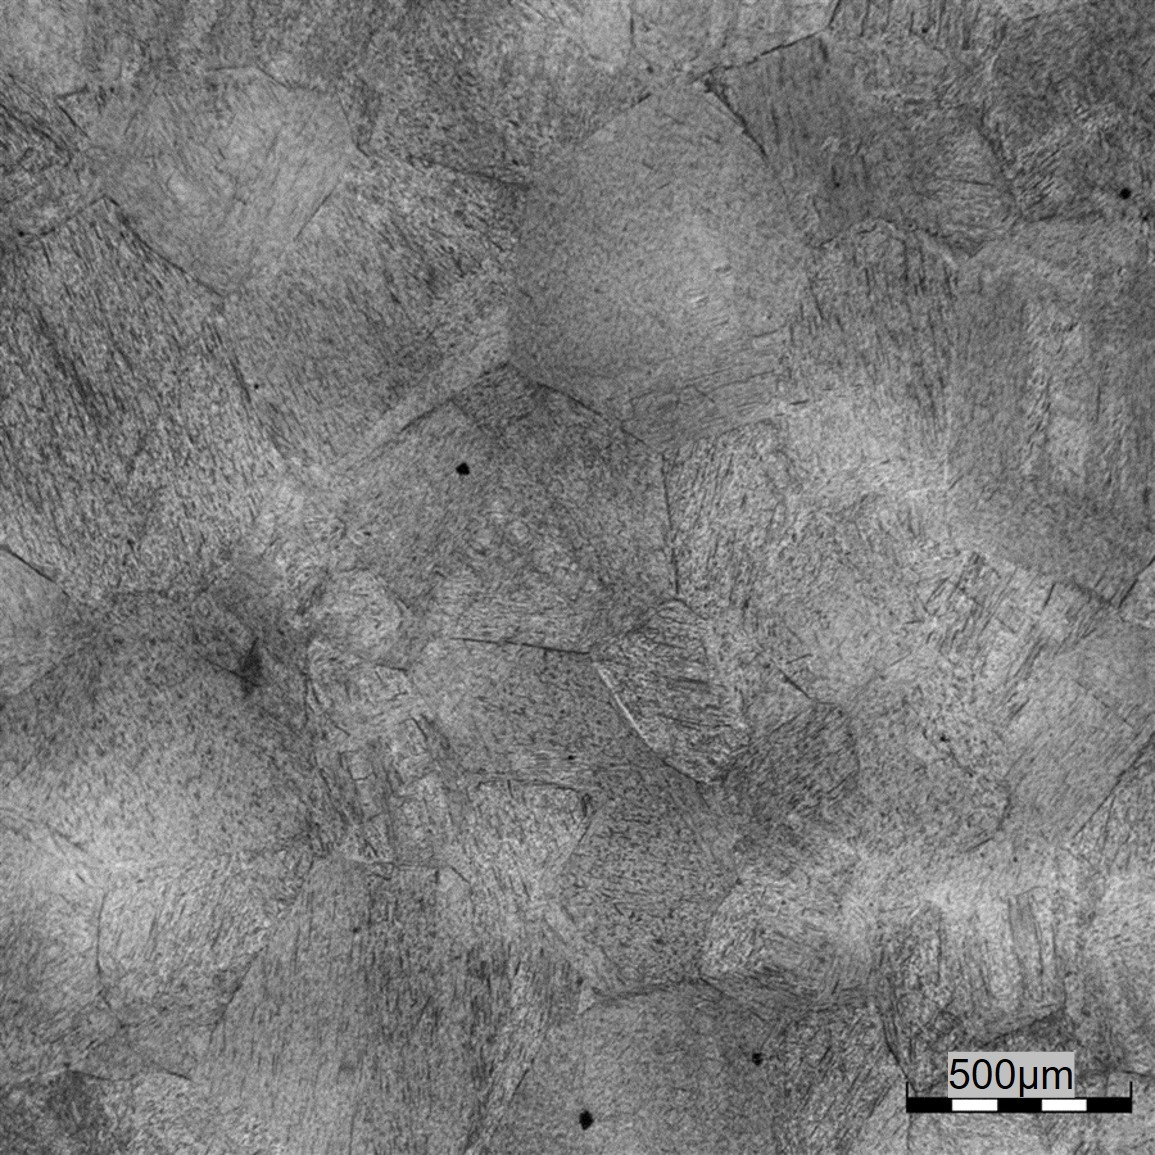
\includegraphics[width=\columnwidth]{Figures/BeforeCompM}
\caption{Before hot compression}
\end{subfigure}
\hfill
\begin{subfigure}[b]{0.45\columnwidth}
\centering
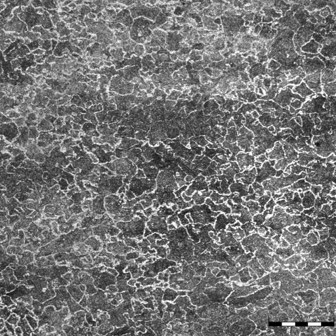
\includegraphics[width=\columnwidth]{Figures/AfterCompM}
\caption{After hot compression}
\end{subfigure}
\caption{Optical micrographs of a medium carbon steel (a) before  and (b) after hot compression.}
\label{fig:Micrography}
\end{figure}
As observed on the flow curves reported in Figure \ref{fig:RawData}, it can be seen by comparing the two micrographs in Figure \ref{fig:Micrography} that recrystallization is almost complete for this temperature and strain rate within the sample held for 5 minutes at $1260^\circ$C and rapidly cooled to get austenitized grain on the one hand, and on the other hand, held for $1$ minute at $1150^\circ$C before compression with a $0.001~\text{s}^{-1}$ strain rate.
The results reported in Figure \ref{fig:RawData},will be used in the next section to identify the parameters of the $6$  proposed flow laws in order to see which mode will matches with experimental.

%----------------------------------------------------------------------------------
\section{Identification of Constitutive Flow Laws Parameters\label{sec:ConstLaws}}
%----------------------------------------------------------------------------------
%----------------------------------------------------------------------------------
\subsection{The Johnson-Cook model\label{sec:JC}}
%----------------------------------------------------------------------------------

The JC model, as mentioned above, is one of the most widely used analytical models because it can be applied to many materials under different conditions of strain $\varepsilon$, strain rate $\mdot\varepsilon$, and temperature $T$.
However, the formulation of this model does not take into account the simultaneous effect of strain, strain rate and temperature.
Indeed, it is formulated by describing the effect of each physical parameter ($\varepsilon$, $\mdot\varepsilon$ and $T$) separately as a factor in the mathematical expression of the model, hence its inability to describe the phenomenon of softening induced by temperature.
The equation that describes this model is given as follows \cite{Johnson-1983}:
\begin{equation}
\sigma^y=\left(A+B\varepsilon^{p^{n}}\right) \left[1+C\ln\left(\frac{\mdot\varepsilon}{\mdot\varepsilon_0}\right)\right] \left[1-\left(\frac{T-T_0}{T_m-T_0}\right)^{m}\right],\label{eq:Johnson-Cook}
\end{equation}
where $\sigma^y$ is the flow stress, $\varepsilon^p$ is the plastic strain, $A$ is the initial elastic limit of the material, $B$is the strain hardening coefficient, $n$ is the strain hardening exponent, $C$ and $m$ are the material constants that describe the strain rate hardening coefficient and the thermal softening coefficient, respectively.
The other values are reference values: $\mdot\varepsilon_0$ is the reference strain rate, $T_m$ and thus $T_0$ are the melting temperature ($1460\celsius$ in our case) and the reference temperature, respectively.
For the determination of the parameters of the analytical models, the reference values for strain rate and temperature are $\mdot\varepsilon_0=0.001~\ps$ and $T_0=1050\celsius$ respectively.

The procedure used to determine the parameters of the Johnson-Cook law is in accordance with the one proposed by He \eal \cite{He-2013}.
This method allows sequentially obtaining the $5$ parameters in the order $A$, $B$, $n$, $C$ and $m$.
Thus, according to the experimental data, the initial elastic limit of the material at the reference strain rate $\mdot\varepsilon_0$ and the reference temperature $T_0$ is $A=13.5143~\MPa$.
For the determination of the constants $B$ and $n$, from the results of the compression test at $T_0$ and $\mdot\varepsilon_0$, these two constants can then determined by considering only the first term $\left(A+B\varepsilon^{p^{n}}\right)$ in Equation (\ref{eq:Johnson-Cook}). Thus, here, $B=21.816~\MPa$ and $n=0.0746$. Once the parameters $A$, $B$ and $n$ are known, the determination of $C$, considering that all the curves at $T=T_0$ then gives $C=0.3404$. Finally, the last parameter $m$ is identified from the curves at $\mdot\varepsilon=\mdot\varepsilon_0$ and from knowledge of the previous parameters and gives $m=0.7057$. All parameters of the Johnson-Cook model are reported in Table \ref{tab:JC}.

\begin{table}[h!]
\centering
\caption{Parameter' values of the Johnson-Cook flow law for a medium carbon steel.}
\begin{tabular}{ccccc}
	\hline
	$A~(\MPa)$ & $B~(\MPa)$ &   $n$    &   $C$    &   $m$    \\
	   $13.5143$     &     $21.816$     & $0.0746$ & $0.3404$ & $0.7057$ \\ \hline
\end{tabular}
\label{tab:JC}
\end{table}

The values predicted by the Johnson-Cook flow law (solid line) and the experimental values (dots) are compared in Figure \ref{fig:CompExp-JC-6}.
\begin{figure}[!ht]
\centering
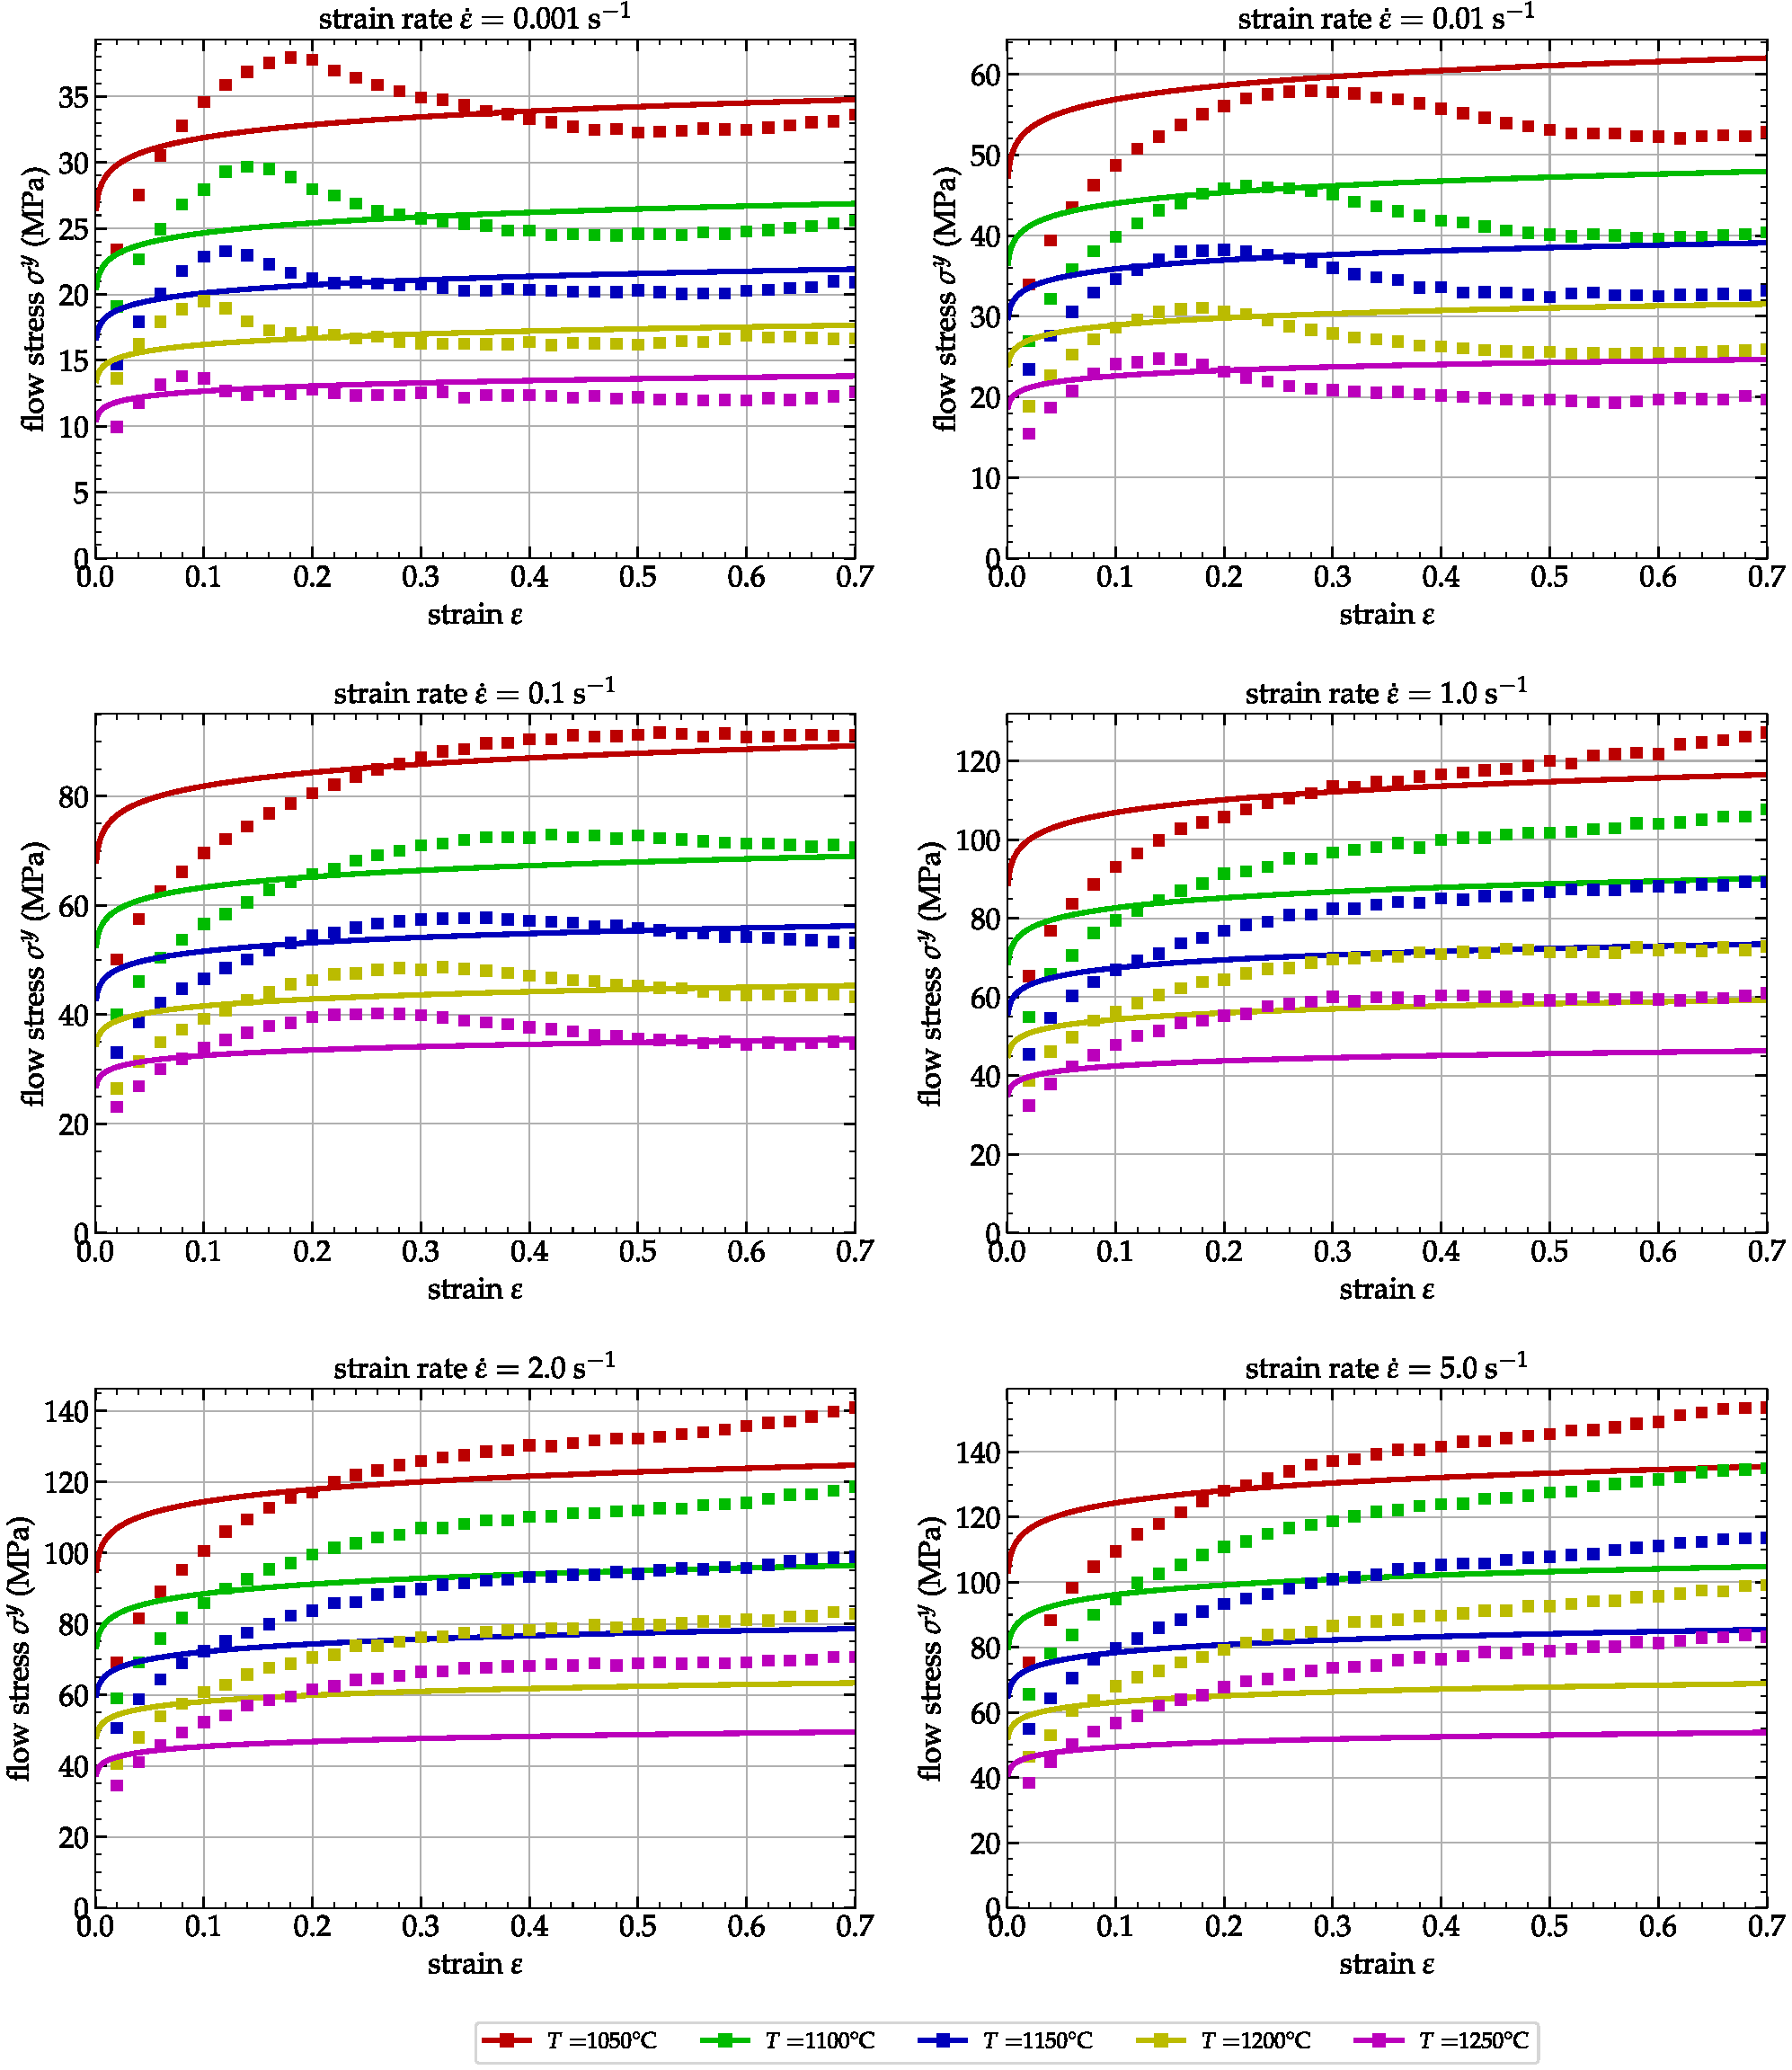
\includegraphics[width=\columnwidth]{Figures/CompExp-JC-6}
\caption{Comparison between the experimental flow stresses and those by JC model.}
\label{fig:CompExp-JC-6}
\end{figure}
The JC model is unable to describe the evolution of the flow stress of medium carbon for all strain values, and the predicted stresses $\sigma^y$ show a monotonically decreasing trend for several strain rates values. The discrepancy between the predicted and experimental values is large for low strains and sometimes acceptable for high strains. As expected, the mathematical formulation of the Johnson-Cook flow law is unable to represent the stress drop at low strain rates, with the JC model increasing only monotonically with the strain. Since most of the parameters are identified at low strain rates ($A$, $B$ and $n$), this results in a very poor fit of the model to the experimental data.

The accuracy and predictive ability of the models are usually assessed through certain coefficients such as the Mean Absolute Relative Error ($\AARE$) defined by Equation (\ref{eq:AARE}):
\begin{equation}
\AARE(\%) = \frac{1}{N} \sum_{i=1}^{N}{\left|\frac{\sigma_i^p -\sigma_i^e}{\sigma_i^e}\right|} \times 100, \label{eq:AARE}
\end{equation}
and the Root Mean Square Error ($\RMSE$) defined by Equation (\ref{eq:RMSE}):
\begin{equation}
\RMSE (\MPa) = \sqrt{\frac{1}{N} \sum_{i=1}^{N} \left(\sigma_i^p - \sigma_i^e\right)^2}, \label{eq:RMSE}
\end{equation}
where $\sigma_i^e$ is the experimental value and $\sigma_i^p$ is the value predicted using the given model of the flow stress $\sigma^y$ and $N$ is the total number of data points used to compute those coefficients (in our case $N=21~000$).
For the JC model, $\AARE=14.05~\%$ and $\RMSE=12.00~\MPa$.
As reported by Phaniraj \cite{Phaniraj-2003}, the correlation coefficient ($\R$) is generally not a good measure in our case of study because it only shows the correlation of the model with respect to the data and not its accuracy, which is a determining factor in the qualification of a model.
Therefore, as a good (high) value of $\R$ (close to $1$) does not necessarily mean a good prediction of the model but simply establishes a good linearity correlation between the experiment and the prediction we avoided its use in our analysis.

%----------------------------------------------------------------------------------
\subsection{The Modified Zerilli-Armstrong model\label{sec:MZA}}
%----------------------------------------------------------------------------------

The MZA which is the modified form of the ZA model, as the JC model is one of widely used models and implemented into many FEM codes like Abaqus software. The difference between the MZA model and JC model is related to the consideration of the three physical parameters to describe the reality observed from experiments. In the JC model, the parameters are considered separately, while in MZA, they are  considered simultaneously and for that formulation, MZA is preferred to the JC model \cite{Hull-2011}.
However, the original form of the ZA model has some limitations due to the fact that it is considered as two terms (thermal and athermal functions), and to improvre formulation, Samantaray \eal \cite{Samantaray-2009} proposed a modified form given by the following equation:
\begin{equation}
\label{eq:MZA-model}
\sigma^y = \left(C_{1}+C_{2}\varepsilon^{p^n}\right) \exp\left[-\left(C_{3}+C_{4}\varepsilon^p\right)\left(T-T_0\right) + \left(C_{5}+C_{6}\left(T-T_0\right)\right)\ln\left( \frac{\mdot\varepsilon}{\mdot{\varepsilon}_0}\right)\right],
\end{equation}
where the $7$ coefficients($C_i$ and $n$) are the parameters of the model to be identified for a given material.
To get the parameters of the MZA model, we apply the method proposed by \cite{Samantaray-2009} and the parameters are summarized in in Table \ref{tab:MZA,} while their predictions are plotted in Figure \ref{fig:CompExp-MZA-6}.
\begin{table}[h!]
\centering{}
\caption{Parameters' constants of Modified-Zerilli-Armstrong model}
\begin{tabular}{ccccccc}
	\hline
	  $C_1$   &   $C_2$   &         $C_3$          &         $C_4$          &  $C_5$   &         $C_6$         &   $n$    \\
	$13.5143$ & $21.2591$ & $4.7902\times 10^{-3}$ & $1.4895\times 10^{-4}$ & $0.1389$ & $1.495\times 10^{-4}$ & $0.0621$ \\ \hline
\end{tabular}
\label{tab:MZA}
\end{table}
\begin{figure}[!ht]
\centering
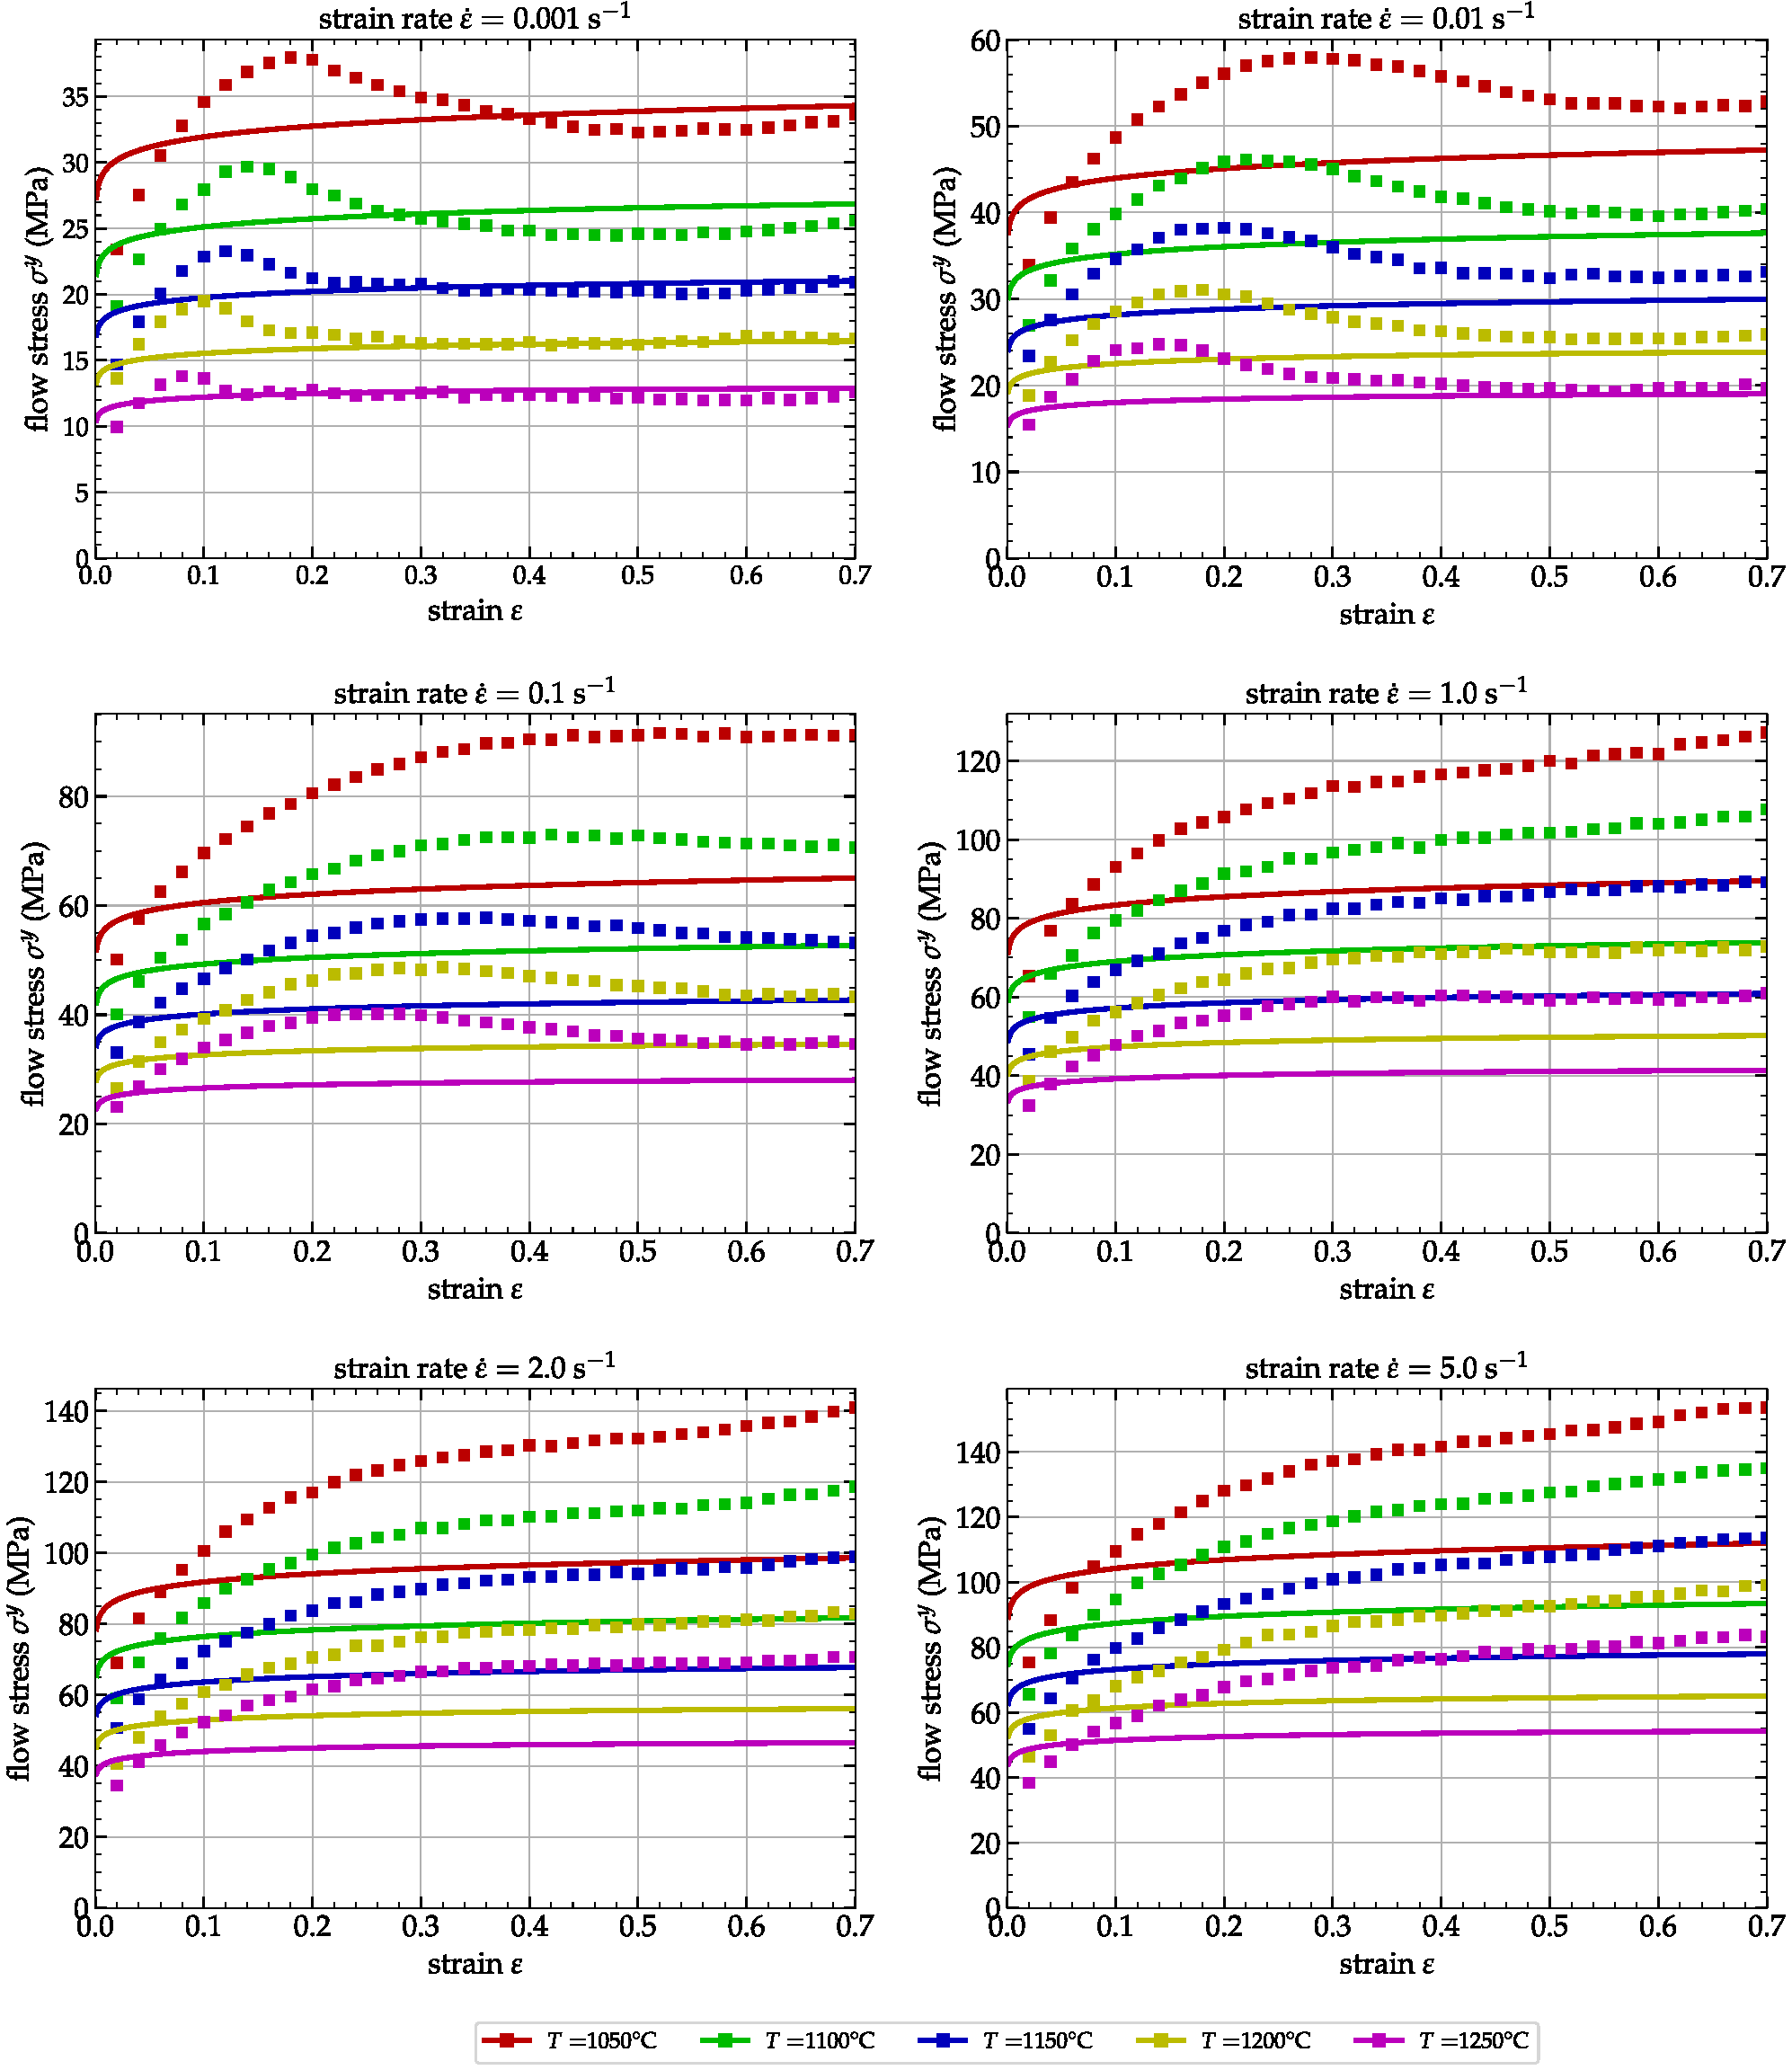
\includegraphics[width=\columnwidth]
{Figures/CompExp-MZA-6}
\caption{Comparison between the experimental flow stresses and those predicted by the MZA model}
\label{fig:CompExp-MZA-6}
\end{figure}
It can be seen from the figures that the MZA model as JC model is not suitable to describe experimental at low strain rates but much better for high strain rates.
The deviation between the predicted values and the experimental values is large because this model has problem correctly describing the softening in its formulation.
For the MZA model, $\AARE=21.20~\%$ and $\RMSE=19.57~\MPa$, showing an overall worse performance than the JC model as reported in \cite{TizeMha-2022}.

%----------------------------------------------------------------------------------
\subsection{The Hansel-Spittel model\label{sec:HSmodel}}
%----------------------------------------------------------------------------------

The Hansel-Spittel model \cite{Hensel-1978} is one of the least known models in terms of integration in FEM codes, although its parameters can more easily be determined than those of the JC or MZA models.
Programming a simple identification script is sufficient to identify its parameters for a given material.
The equation of the HS model is given by the following relation:
\begin{equation}
\sigma^y = A~\e{m_1T}~\varepsilon^{m_2}~\mdot\varepsilon^{m_3}~\e{({m_4}/{\varepsilon})}~(1+\varepsilon)^{m_5T}~\e{m_6\varepsilon}~\mdot\varepsilon^{m_7T}~T^{m_8}, \label{eq:HS}
\end{equation}
where again, $\sigma^y$ is the flow stress, $\varepsilon$ is the strain, $\mdot\varepsilon$ is the strain rate and $T$ is the temperature as proposed earlier.
The coefficients $A$ and $m_i$ are the 9 parameters of the model to be identified.
However, this model has some shortcomings, notably related to the fact that its accuracy varies according to the number of parameters taken into account during the identification.
For its identification, several authors restrict its expression to a reduced number of only $5$ or $6$ $m_i$ parameters, by forcing a zero value for the other parameters \cite{Chadha-2018, Mehtedi-2015, Rudnytskyj-2020}.

In the present study, the best results were obtained by taking the model defined by only the first 7 $m_i$ terms of the equation (\ref{eq:HS}), so that $m_8=0$.
From the experimental data obtained during the compression tests, an identification procedure based on the use of the LMFIT optimizer \cite{Newville-2016} allowed to compute the parameters reported in Table 
 \ref{tab:HS}.

\begin{table}[h!]
\centering
\caption{Parameters' values of the Hansel-Spittel flow law for the medium carbon steel.}
\begin{tabular}{ccccc}
	\hline
	        $A$          &         $m_1$          &   $m_2$   &        $m_3$         &         $m_4$         \\
	$5.954\times 10^{3}$ & $-3.3576\times10^{-3}$ & $0.2641$  &      $-0.0868$       & $2.2688\times10^{-4}$ \\ \hline
	                     &         $m_5$          &   $m_6$   &        $m_7$         &         $m_8$         \\
	                     & $-4.2163\times10^{-4}$ & $-0.0561$ & $2.264\times10^{-4}$ &          $0$          \\ \hline
\end{tabular}
\label{tab:HS}
\end{table}

A comparison of the values predicted by the HS model and the experimental values is presented in Figure \ref{fig:CompExp-HS-6}, where the dots represent the experimental values and the solid lines are the values predicted by the Hansel-Spittel flow law.
For the HS model, $\AARE=7.75~\%$ and $\RMSE=3.80~\MPa$.
It appears that both this model and the previous ones do not adequately predict the experimental one, and the difference is relatively significant for all strain rates below $1~\ps$.
This shows that this model is not appropriate for the characterization of this alloy, particularly because of the strong non-linear the behavior observed for low strain rate values. The DRX phenomenon cannot be reproduced by this type of model.

\begin{figure}[!ht]
\centering
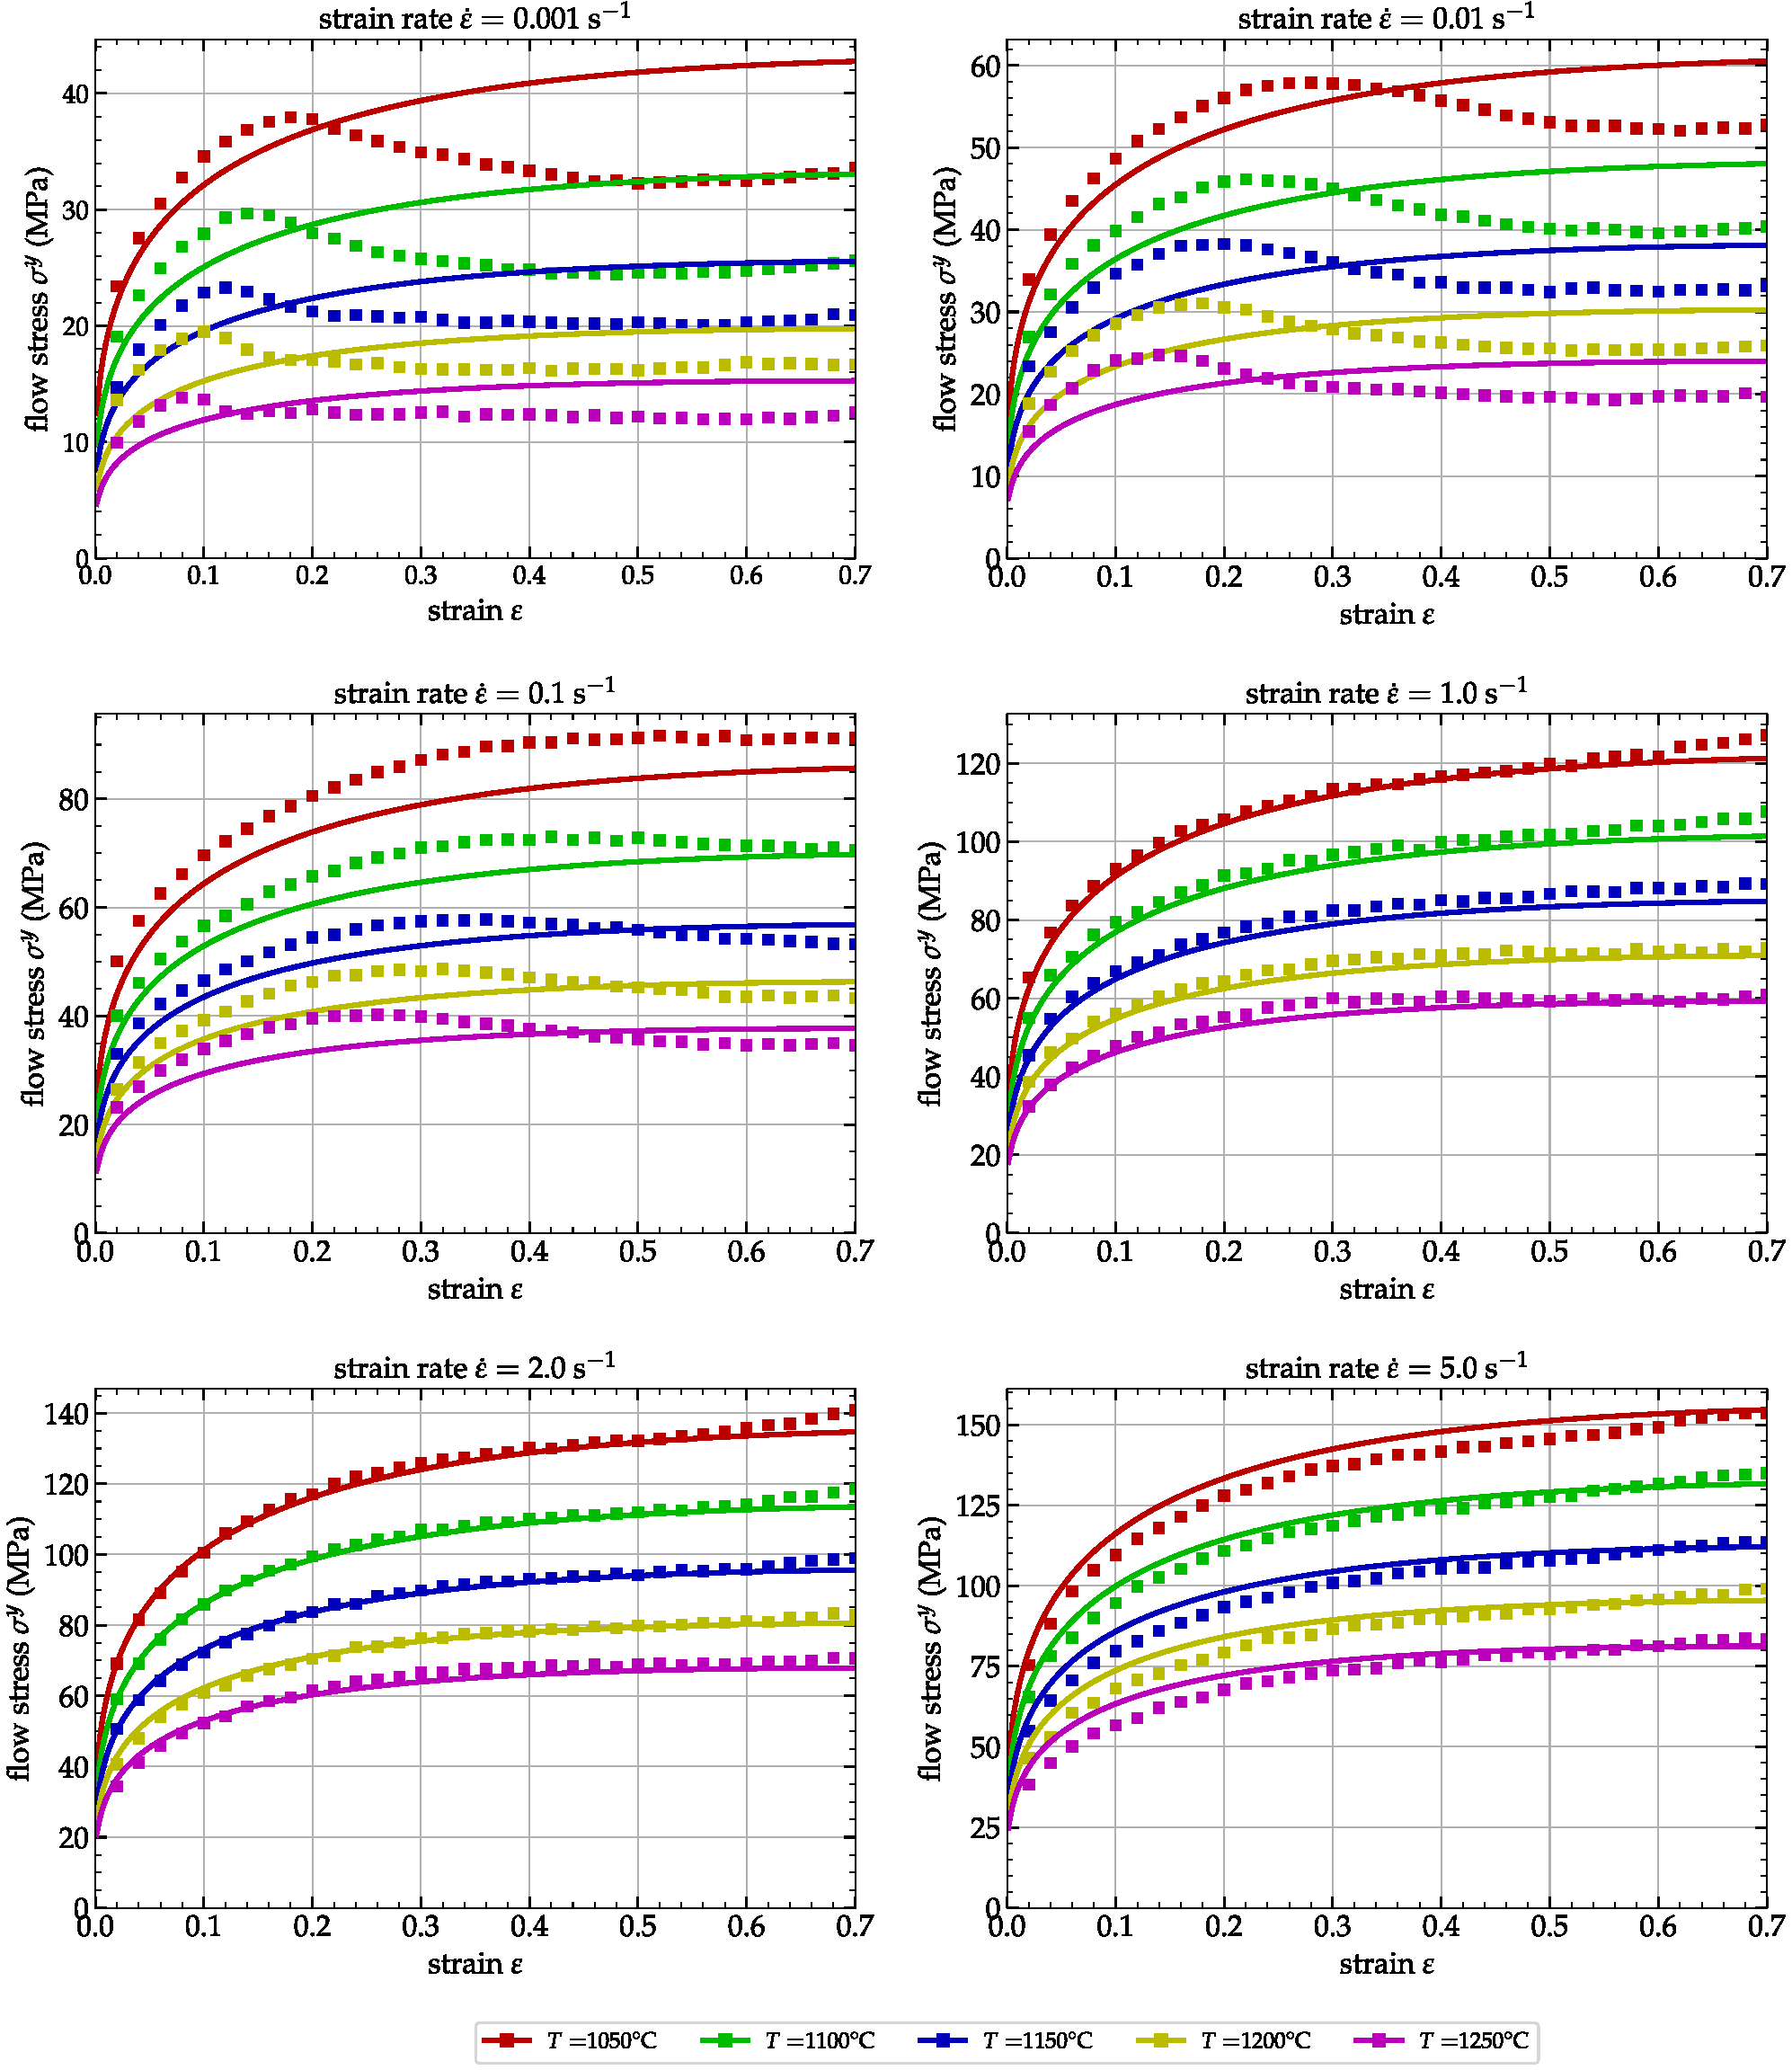
\includegraphics[width=\columnwidth]
{Figures/CompExp-HS-6}
\caption{Comparison between the experimental flow stresses and those predicted by the HS model}
\label{fig:CompExp-HS-6}
\end{figure}

%----------------------------------------------------------------------------------
\subsection{The Arrhenius model\label{sec:ARmodel}}
%----------------------------------------------------------------------------------

The Arrhenius type model \cite{Sellars-1966} is one of the most used models in the framework of material forming, especially when it comes to studying the material microstructure.
The model takes into account the physical phenomena describing the behavior of the material in the formulation of the relationships between the stress $\sigma^y$, the strain $\varepsilon$, the strain rate $\mdot\varepsilon$ and the temperature $T$ expressed as power law, exponential law and hyperbolic sine.
This makes it easier to describe the softening phenomenon observed in the material due to increasing temperature.
The following equations describe the Arrhenius model:
\begin{equation}
\mdot\varepsilon =
\begin{cases}
A_1 \sigma^{y^{n_1}} \exp{\left(-\frac{Q}{RT}\right)} & \alpha\sigma^y < 0.8\\
A_2 \exp(\beta\sigma^y) \exp{\left(-\frac{Q}{RT}\right)} & \alpha\sigma^y > 1.2\\
A_3 \left[\sinh{\left(\alpha\sigma^y\right)}\right]^{n_2} \exp{\left(-\frac{Q}{RT}\right)} & \text{for all }\sigma^y
\end{cases}
\label{eq:ArDef}
\end{equation}
with:
\begin{equation}
Z = \mdot\varepsilon \exp{\left(\frac{Q}{RT}\right)}, \label{eq:ArZ}
\end{equation}
Where $Z$ is the Zenner-Hollomon parameter \cite{Zener-1944}, $\mdot\varepsilon$ is the strain rate ($\ps$), $Q$ is the apparent activation energy ($\text{J~mol}^{-1}$), $R$ is the universal gas constant ($8.314~\text{J~mol}^{-1} \text{K}^{-1}$), $T$ is the absolute temperature (K), $\sigma^y$ is the flow stress (MPa) for a given strain, strain rate and temperature and $A_1$, $A_2$, $A_3$, $n_1$, $n_2$, $\alpha$ and $\beta=\alpha~n_1$ are dependent on the material. The corresponding values are independent of the temperature and are obtained from the stress-strain curves at different strain rates and temperatures by the regression method. Combining Equations (\ref{eq:ArDef}) and (\ref{eq:ArZ}) allows to express the flow stress $\sigma^y$ as a function of the $Z$ parameter:
\begin{equation}
\sigma^y = \frac{1}{\alpha} \ln\left\{\left(\frac{Z}{A}\right)^{1/n} + \left[1 + \left(\frac{Z}{A}\right)^{2/n}\right]^{1/2}\right\}
\end{equation}

To obtain the constitutive equation, all the parameters $A$, $Q$ $\alpha$ and $n$must be determined for a given material. The strain has a significant non-linear influence on the behavior of the material by the  strain hardening and softening mechanisms at high values of deformation.
A strain dependent factor must therefore be taken into account in the Arrhenius model, which leads to the definition of the modified Arrhenius model for which the $A$, $Q$ $\alpha$ and $n$ parameters are expressed as a function of the strain $\varepsilon$ by means of polynomial functions of degree $m$ (varying from $1$ to $9$) of the form:
\begin{equation}
A(\varepsilon) = \exp{\left[\ln\!A_0 + \ln\!A_1\varepsilon + \ln\!A_2\varepsilon^2 + \ln\!A_3\varepsilon^3 + \cdots + \ln\!A_m\varepsilon^m\right]}
\label{eq:ArA}
\end{equation}
\begin{equation}
Q(\varepsilon) = Q_0 + Q_1\varepsilon + Q_2\varepsilon^2 + Q_3\varepsilon^3 + \cdots + Q_m\varepsilon^m
\label{eq:ArQ}
\end{equation}
\begin{equation}
\alpha(\varepsilon) = \alpha_0 + \alpha_1\varepsilon + \alpha_2\varepsilon^2 + \alpha_3\varepsilon^3 + \cdots + \alpha_m\varepsilon^m
\label{eq:Aralpha}
\end{equation}
\begin{equation}
n(\varepsilon) = n_0 + n_1\varepsilon + n_2\varepsilon^2 + n_3\varepsilon^3 + \cdots + n_m\varepsilon^m
\label{eq:Arn}
\end{equation}

The determination of the order $m$ of the polynomials defined by Equations (\ref{eq:ArA}-\ref{eq:Arn}) is defined according to the ability of the model to represent the non-linear dependence of the stress versus the strain and its generalization.
The values $\ln\!A_i$, $\alpha_i$, $n_i$, and $Q_i$ ($i=0,1,2,3,\cdots,m$) are the coefficients of the polynomials used to determine using a regression method.
Setting $m=9$ gives the best results and the corresponding parameters are reported in Table \ref{tab:AR}.
\begin{table}[h!]
\centering
\caption{Parameters' values of the Arrhenius flow law for the medium carbon steel.}
\begin{tabular}{llll}
	\hline
	\multicolumn{1}{c}{$\alpha_i$}  & \multicolumn{1}{c}{$Q_i~(\times 10^{-6})$} & \multicolumn{1}{c}{$\ln\!A_i$} & \multicolumn{1}{c}{$n_i$}  \\ \hline
	$\alpha_0=0.0407$               & $Q_0=0.467$                                & $A_0=35.8092$                  & $n_0=4.8217$               \\
	$\alpha_1=-0.5167$              & $Q_1=-0.6517$                              & $A_1=-58.822$                  & $n_1=3.2814$               \\
	$\alpha_2=6.3912$               & $Q_2=7.6084$                               & $A_2=740.3303$                 & $n_2=71.5963$              \\
	$\alpha_3=-47.3364$             & $Q_3=-48.016$                              & $A_3=-5.0493\times 10^{3}$     & $n_3=-1.9562\times 10^{3}$ \\
	$\alpha_4=220.0014$             & $Q_4=66.795$                               & $A_4=1.1305\times 10^{4}$      & $n_4=1.4461\times 10^{4}$  \\
	$\alpha_5=-654.4553$            & $Q_5=468.8898$                             & $A_5=2.022\times 10^{4}$       & $n_5=-5.431\times 10^{4}$  \\
	$\alpha_6=1.2421\times 10^{3}$  & $Q_6=-2.3032\times 10^{3}$                 & $A_6=-1.5387\times 10^{5}$     & $n_6=1.1761\times 10^{5}$  \\
	$\alpha_7=-1.4523\times 10^{3}$ & $Q_7=4.3707\times 10^{3}$                  & $A_7=3.1798\times 10^{5}$      & $n_7=-1.4882\times 10^{5}$ \\
	$\alpha_8=952.0619$             & $Q_8=-3.9394\times 10^{3}$                 & $A_8=-2.9725\times 10^{5}$     & $n_8=1.0239\times 10^{5}$  \\
	$\alpha_9=-267.4994$            & $Q_9=1.397\times 10^{3}$                   & $A_9=1.0759\times 10^{5}$      & $n_9=-2.9621\times 10^{4}$ \\ \hline
\end{tabular}
\label{tab:AR}
\end{table}
This modified form of the Arrhenius behavior law allows an accurate and reliable prediction over a wide range of temperatures and strain rates.
Equation (\ref{eq:ArStress}) is finally used to compute the flow stress $\sigma^y$ from the strain $\varepsilon$, the strain rate $\mdot\varepsilon$ and the temperature $T$:
\begin{equation}
\sigma^y = \frac{1}{\alpha(\varepsilon)} \ln\left\{\left(\frac{\mdot\varepsilon \exp{\left(\frac{Q(\varepsilon)}{RT}\right)}}{A(\varepsilon)}\right)^{\frac{1}{n(\varepsilon)}} + \left[1 + \left(\frac{\mdot\varepsilon \exp{\left(\frac{Q(\varepsilon)}{RT}\right)}}{A(\varepsilon)}\right)^{\frac{2}{n(\varepsilon)}}\right]^{\frac{1}{2}}\right\}
\label{eq:ArStress}
\end{equation}

Figure \ref{fig:CompExp-AR-6} shows a comparison of the values predicted by the Arrhenius model and the experimental values. The difference between the experimental and predicted values is small. However for the strain rate $\mdot\varepsilon = 0.01~\ps$ and for the two low temperature values, the AR model is unable to predict the softening. For the AR model, $\AARE=3.56~\%$ and $\RMSE=2.18~\MPa$.
\begin{figure}[!ht]
\centering
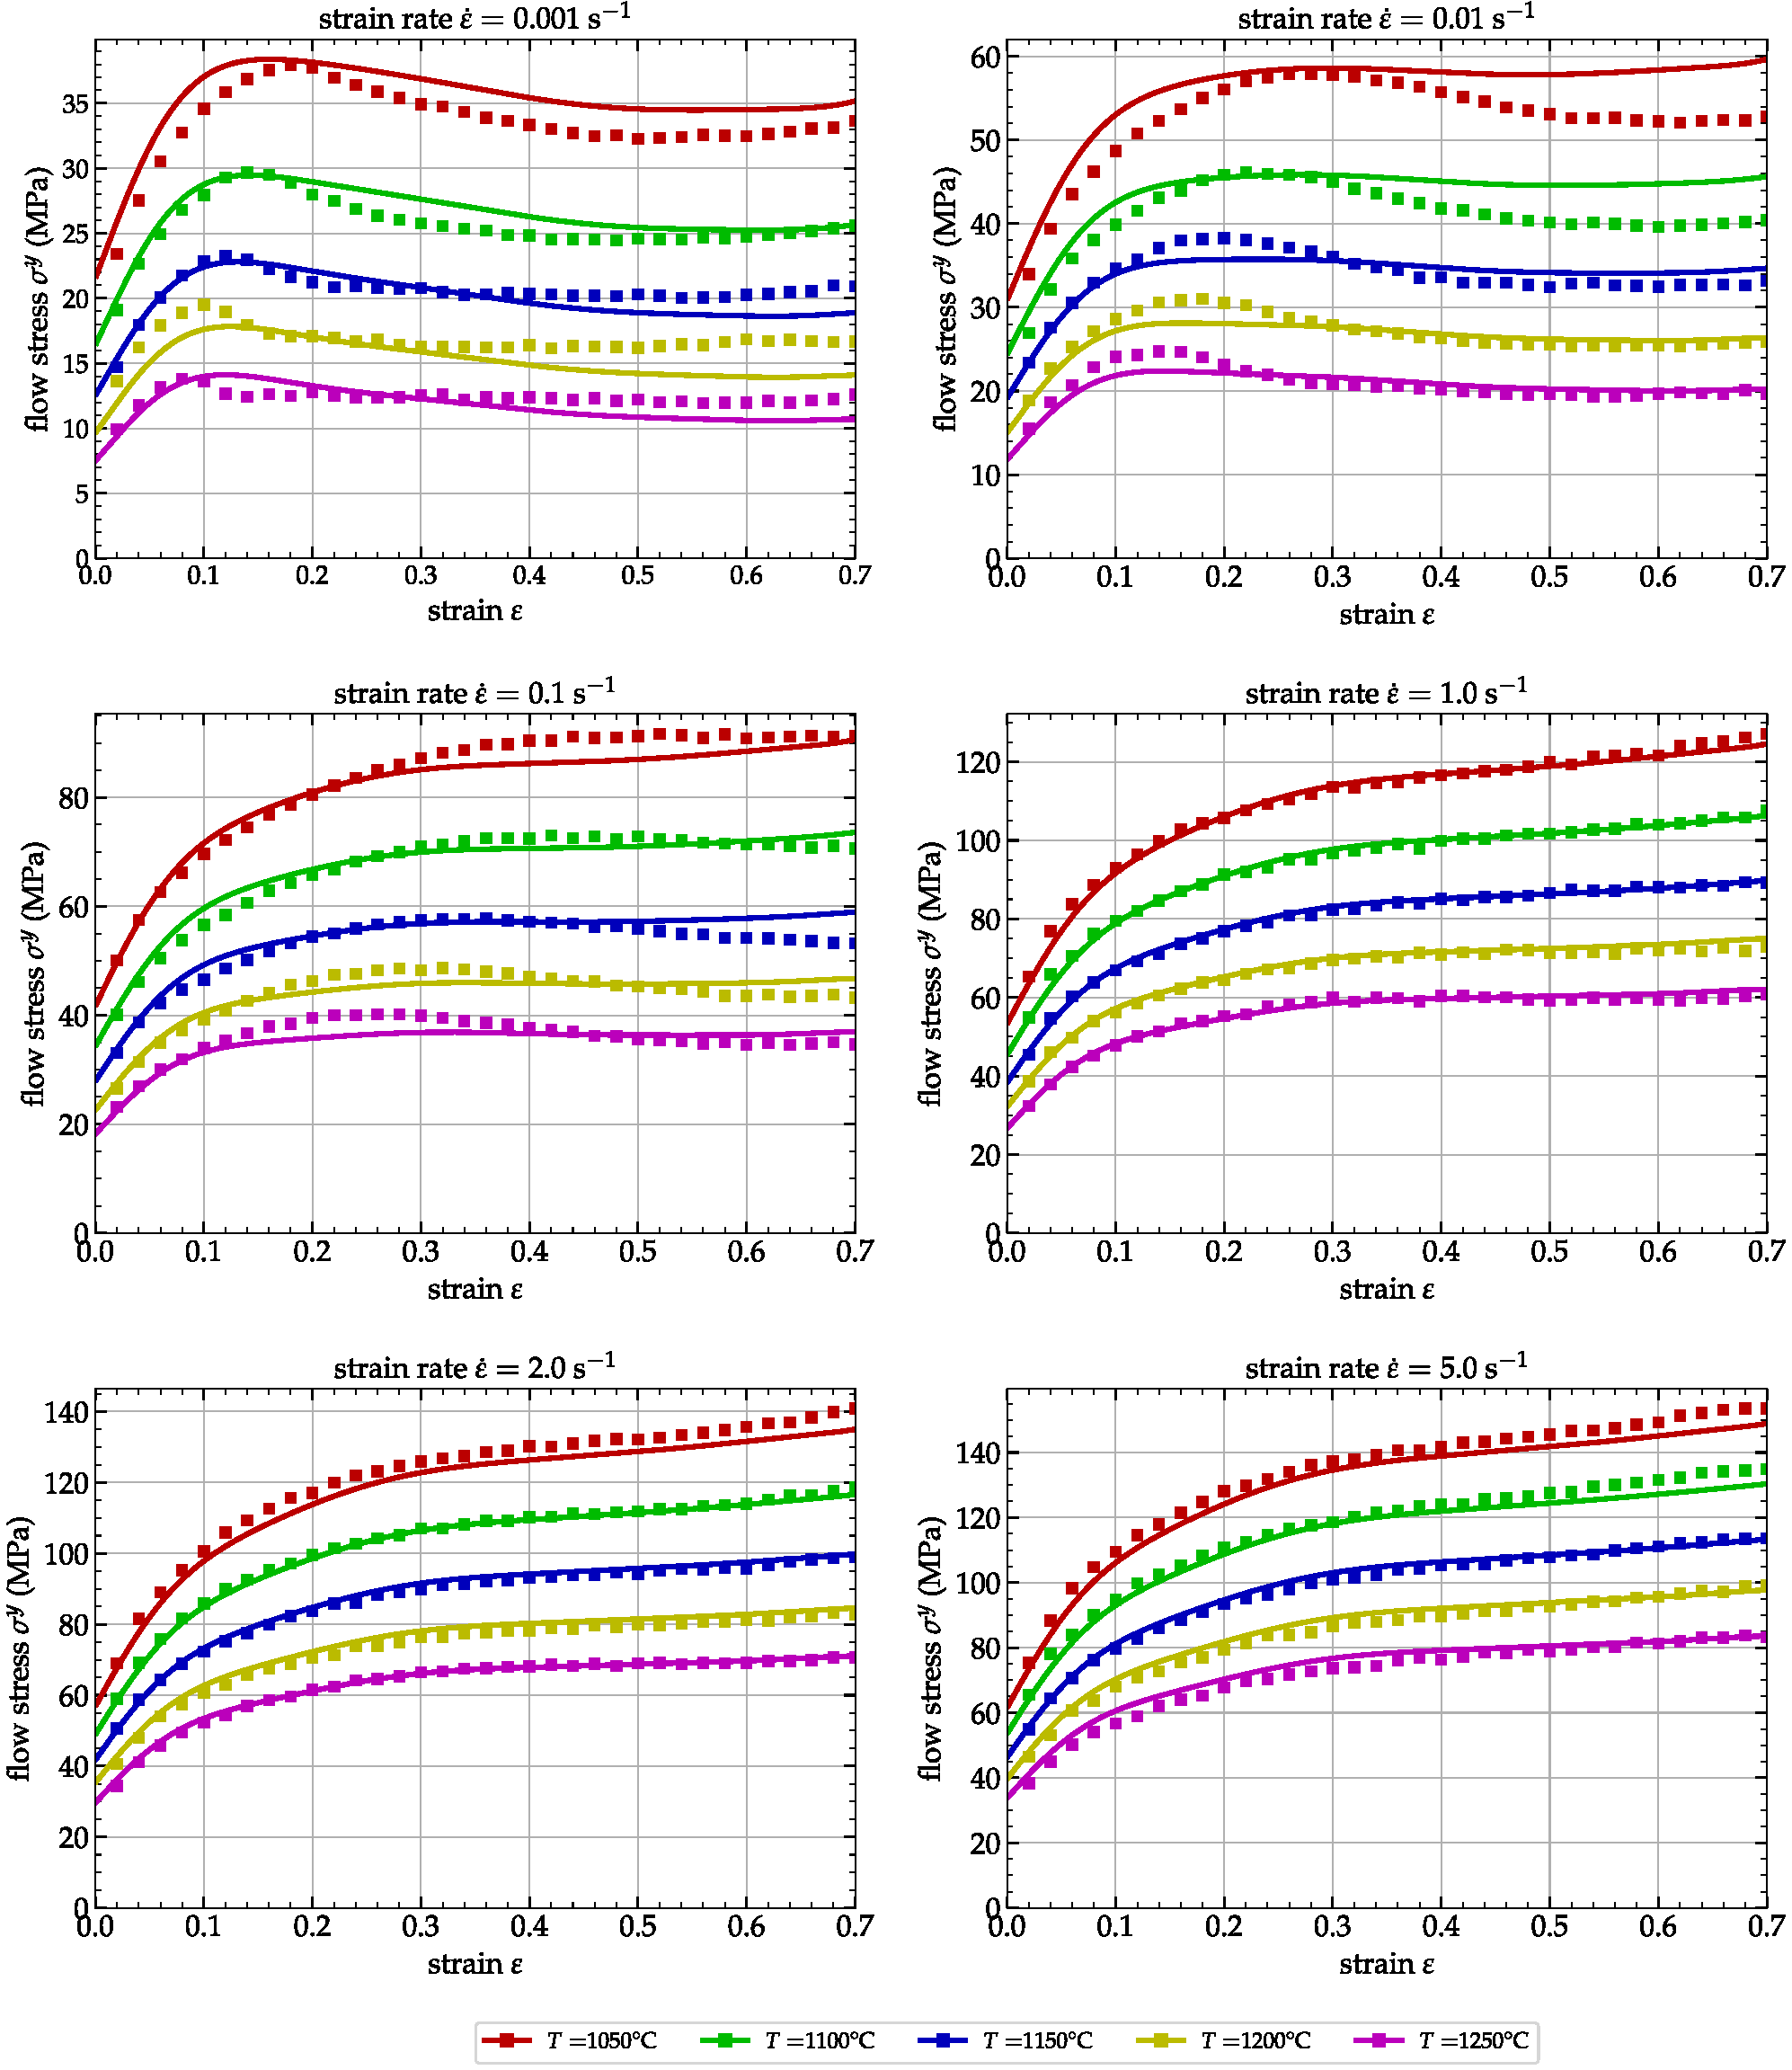
\includegraphics[width=\columnwidth]
{Figures/CompExp-AR-6}
\caption{Comparison between the experimental flow stresses and those predicted flow stresses by the AR model}
\label{fig:CompExp-AR-6}
\end{figure}

%----------------------------------------------------------------------------------
\subsection{The PTM model\label{sec:PTM}}
%----------------------------------------------------------------------------------

The PTM model \cite{TizeMha-2022} is a generalized formulation of the MZA model presented in Section \ref{sec:MZA}.
When establishing its formulation, the main shortcomings of the MZA model were taken into account, in order to render the PTM model flexible for any type of material studied because it removes need for a limited number of parameters as in the MZA model. Its construction is based on the use of polynomial functions, as is the case in the AR model. Thus, the physical parameters' dependent intrinsic functions of the PTM model, allow adjusting the model according to the degree selected for each of the 4 constituent polynomials, which provides a good fit for each function.
The equation describing the PTM model is therefore given by :
\begin{equation}
\label{eq:PTM-model}
\sigma^y = \left(\sum_{i=0}^{q}{A_i\varepsilon^{p^i}}\right) \exp\left[\left(\sum_{j=0}^{r}{B_j\varepsilon^{p^j}}\right)\left(T-T_0\right) + \left(\sum_{k=0}^{s}\left(\sum_{l=0}^{t}{C_k^l\varepsilon^{p^l}} \right)\left(T-T_0\right)^k \right)\ln\left( \frac{\mdot\varepsilon}{\mdot{\varepsilon}_0}\right)\right]
\end{equation}
where $A_i, B_j, C_k^l$ are the parameters (Table \ref{tab:PTM}) of the model to be identified using the procedure proposed in  \cite{TizeMha-2022}.
Quantities $q$, $r$, $s$ and $t$ define the degree of the polynomials used to describe the behavior of the material.
The larger these quantities, the greater the number of parameters needing to be identified for the PTM model. The determination of the parameters of this model is calculated thanks to the LMFIT Python library \cite{Newville-2016} (for more details about this model  we refer the reader to our previous work \cite{TizeMha-2022}). Thus, all the parameters of this model are calculated with $q=5$, $r=5$, $s=1$ and $t=5$.

\ref{fig:CompExp-PTM-6} presents a Comparison of values predicted by the PTM model and experimental values.
The PTM model is suitable for describing the flow behavior of medium carbon steel, but for the two strain rates $\mdot\varepsilon=0.01~\ps$ and $\mdot\varepsilon=0.1~\ps$, the prediction is not very good.
The deviation between the predicted values and the experimental values for other strain rates is relatively low. For the PTM model, $\AARE=4.79~\%$ and $\RMSE=4.59~\MPa$, which is an overall worse performance than the AR model.

\begin{table}[h!]
\centering
\caption{Parameters' values of the PTM flow law for the P20 steel.}
\begin{tabular}{llll}
	\hline
	\multicolumn{1}{c}{$A_i$}  & \multicolumn{1}{c}{$B_i$}   & \multicolumn{1}{c}{$C_0^i$} & \multicolumn{1}{c}{$C_1^i$}   \\ \hline
	$A_0=16.8529$              & $B_0=-3.5418\times 10^{-3}$ & $C_0^0=0.1608$              & $C_1^0=-1.9037\times 10^{-5}$ \\
	$A_1=340.6451$             & $B_1=-0.0132$               & $C_0^1=-0.6202$             & $C_1^1=2.67\times 10^{-3}$    \\
	$A_2=-1.9594\times 10^{3}$ & $B_2=-4.4888\times 10^{-3}$ & $C_0^2=4.9516$              & $C_1^2=-3.5788\times 10^{-3}$ \\
	$A_3=4.836\times 10^{3}$   & $B_3=0.2218$                & $C_0^3=-13.1694$            & $C_1^3=-0.0222$               \\
	$A_4=-5.5176\times 10^{3}$ & $B_4=-0.4988$               & $C_0^4=15.25$               & $C_1^4=0.0609$                \\
	$A_5=2.4058\times 10^{3}$  & $B_5=0.3211$                & $C_0^5=-6.587$              & $C_1^5=-0.0413$               \\ \hline
\end{tabular}
\label{tab:PTM}
\end{table}

\begin{figure}[!ht]
\centering
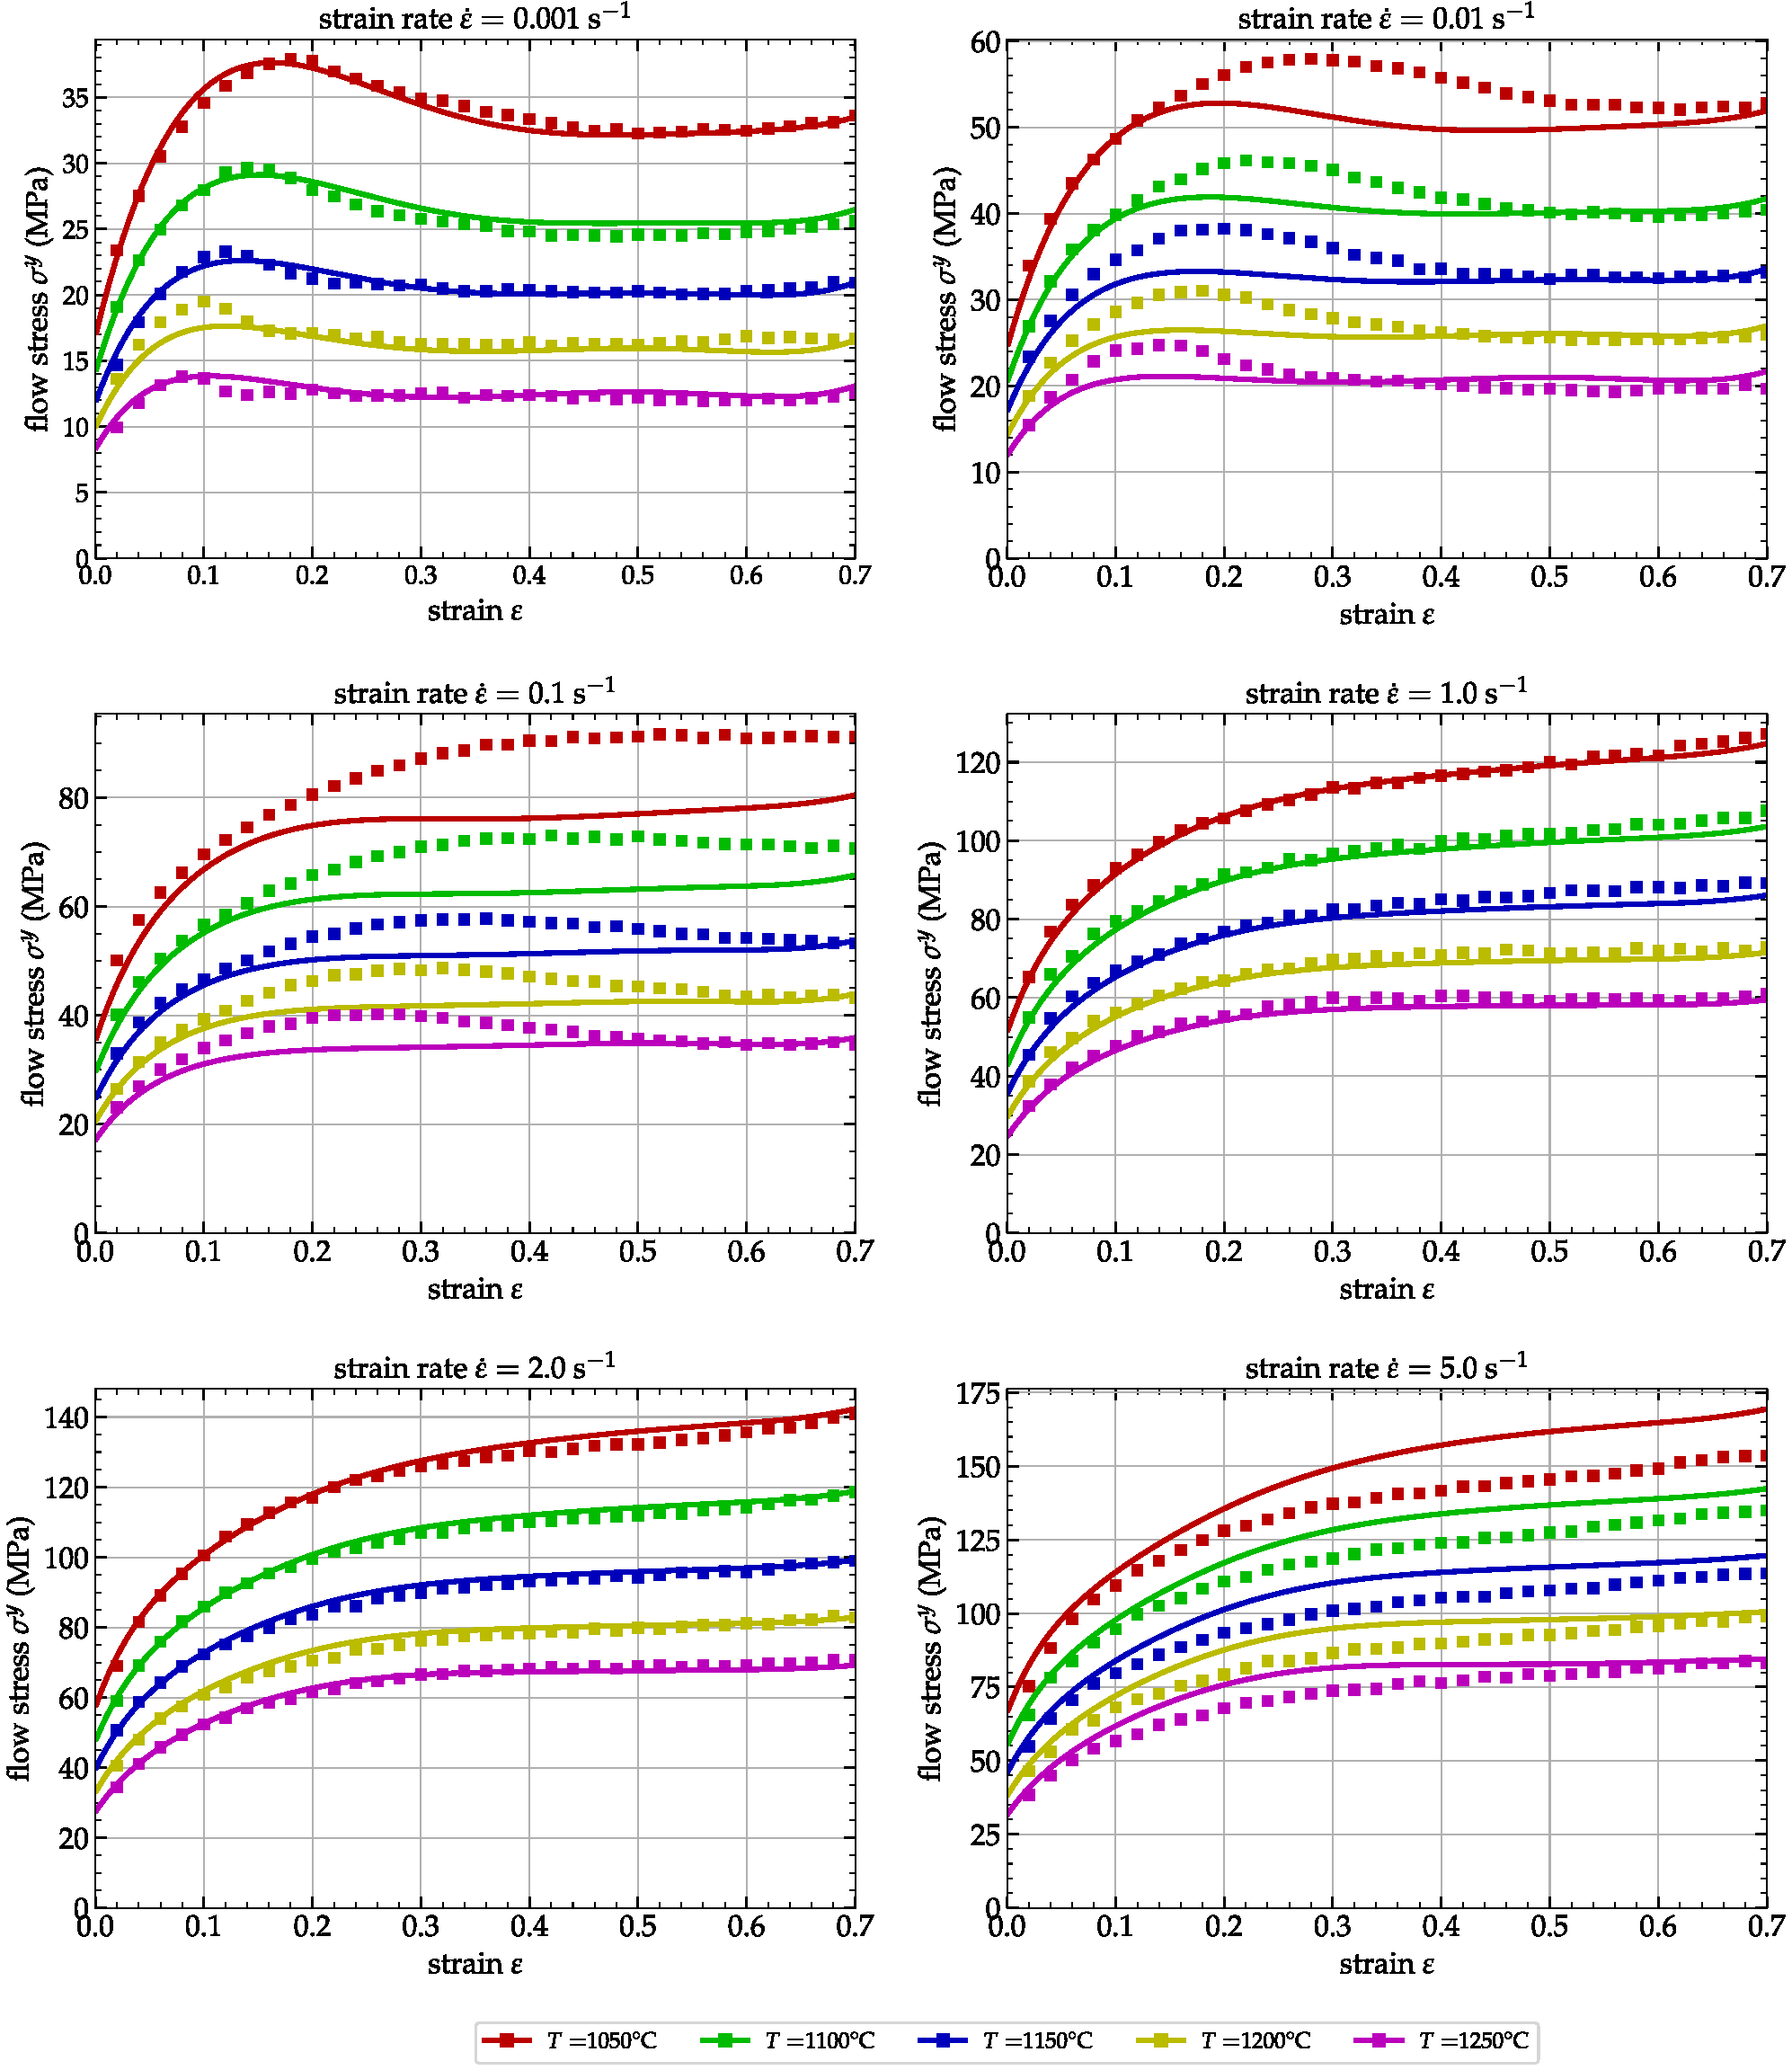
\includegraphics[width=\columnwidth]
{Figures/CompExp-PTM-6}
\caption{Comparison between the experimental flow stresses and those predicted the PTM model}
\label{fig:CompExp-PTM-6}
\end{figure}

%----------------------------------------------------------------------------------
\subsection{The Artificial Neural Network model\label{sec:ANNmodel}}
%----------------------------------------------------------------------------------

Because of their predictive capacity and adaptability, Artificial Neural Networks (ANNs) are increasingly widely used today in many scientific fields. Their operation is based on a learning process during which the principle of minimizing the error between the model's output and the training data allows the adjustment of the model's parameters, as in any machine learning process.

Neural networks generally have two uses: classification and regression.
The first is the ability to classify data into different groups and for example to distinguish between images of cats and dogs. The second corresponds to the universal approximation capacity of these neural networks, which if of interest to us here in, and thus, to the ability, after learning to predict the flow stress $\sigma^y$ values according to the input data, akin to what is done by  the previously identified analytical models. 
The main difference is that this approximation is not linked to a fixed mathematical formulation (JC, MZA, AR, HS, PTM model), but is only dependent on the data used for training, the number of layers, the number of neurons per layer and the activation functions associated with the neurons of the network.
A feed-forward ANN, as used in our application, contains an input layer, an output layer and a number of hidden layers ($2$ in our case).
Each layer of neurons is connected to the one before it and the one after it by weighted connections.
Thus, all the neurons of the $k$ layer are connected to all the neurons of the ($k-1$) layer as shown in Figure \ref{fig:ANN-2HL}.
\begin{figure}[!ht]
\centering
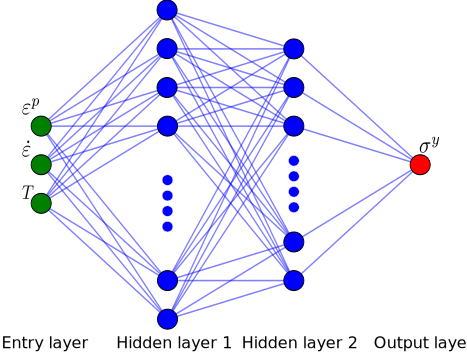
\includegraphics[width=0.7\columnwidth]
{Figures/ANN-scheme-2HL}
\caption{Multi-layer Artificial Neural Network architecture}
\label{fig:ANN-2HL}
\end{figure}

Any hidden layer $k$, containing $n$ neurons, takes a weighted sum of the outputs $\overrightarrow{\hat{y}}$ of the immediately preceding layer $(k-1)$, containing $m$ neurons, given by the following equation:
\begin{equation}
y_i\lay{k} = \sum_{j=1}^m w_{ij}\lay{k} \hat{y}_j^{(k-1)}+ b_i\lay{k},\label{eq:ANN1}
\end{equation}
where $y_i\lay{k}$ is the entry of the $i^{th}$ neuron of layer $k$, $\hat{y}_j\lay{k-1}$ is the output of the $j^{th}$ neuron of layer $(k-1)$, $w_{ij}\lay{k}$ is the associated weight parameter between the $i^{th}$ neuron of layer $k$ and the $j^{th}$ neuron of layer $(k-1)$ and $b_i\lay{k}$ is the associated bias of the $i^{th}$ neuron of layer $k$.
Those weights $w_{ij}$ and bias $b_i$, for each layer, are the training parameters of the ANN which we have to adjust during the training procedure described in Pantalé \eal \cite{Pantale-2021}.
For the proposed model, we selected the Sigmoid activation function, so that, each neuron in the hidden layer $k$ provides an output value ${\hat{y}}$ from the input value $y$ of the same neuron defined by Equation (\ref{eq:ANN1}) according to the following equation:
\begin{equation}
\hat{y}=\frac{1}{1 + \e{-y}}\label{eq:ANN2}
\end{equation}
No activation function is used for the output neuron of the ANN.

After some tests of different types of network architecture and in accordance with previous works, a network structure with two hidden layers including $15$ neurons for the first hidden layer and 7 neurons for the second layer give the best compromise between prediction, learning time and model compactness.
From a global architecture point of view, the input layer is composed of $3$ neurons ($\varepsilon^p$, $\mdot\varepsilon$, $T$) and the output layer is composed of a single neuron corresponding to the $\sigma^y$ flow stress.
This architecture leads to a global model with $180$ parameters to be identified ($60$ for the first layer, $112$ for the second layer and 8 for the output layer).

The Python program used for training the neural network was developed using the specialized Python library Tensorflow \cite{Abadi-2016}.
The Adaptive Moment Estimation (ADAM) optimizer \cite{Kingma-2015} was used for the training phase.
The training data were those from the tests presented in Section \ref{sec:ComTestResults} and were composed of $21~000$ quadruplets of ($\varepsilon^p$, $\mdot\varepsilon$, $T$, $\sigma^y$) values.
The learning was performed on the basis of $5~000$ epochs of the experimental data set.
$40$ minutes of training on a Dell XPS-13 7390 laptop running Ubuntu 22.04 LTS 64 bits with 16 GB of Ram and an Intel 4-core i7-10510U processor allowed to obtain the converged parameters of the ANN model.
Figure \ref{fig:ANN-6-conv} shows the evolution of the training error defined by the $\log_{10}$ of the $\RMSE$  during the training phase.
\begin{figure}[!ht]
\centering
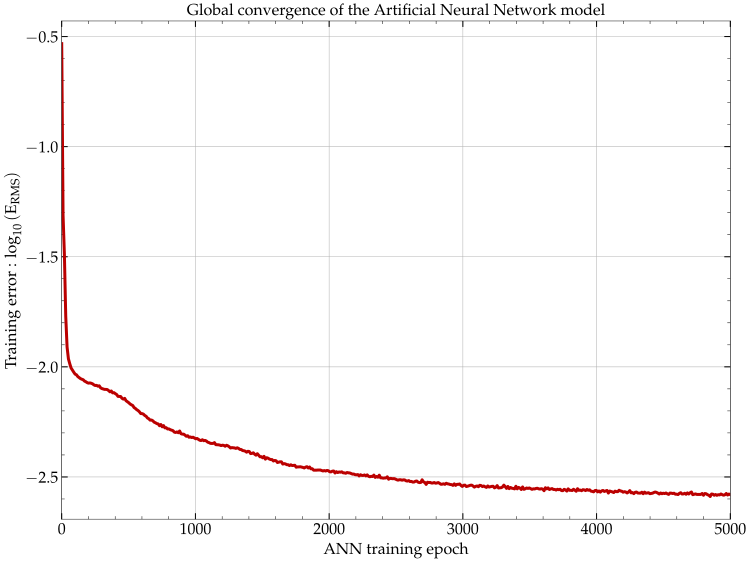
\includegraphics[width=0.7\columnwidth]
{Figures/Conv-ANN-6}
\caption{Convergence of the ANN model during the training phase.}
\label{fig:ANN-6-conv}
\end{figure}
As can be seen in this figure, after $5~000$ epoch, we can consider that we have reached a stationary state of the model learning and that it is useless to continue with the learning phase.

Once the learning phase is over, the trained model can be used to predict the behavior of the medium carbon alloy as a function of the input data similarly to what is done with analytical models.
One can either use the model directly by providing it with new input data, or retrieve the $180$ parameters identified during the training and inject them into a mathematical model based on Equations (\ref{eq:ANN1}) and (\ref{eq:ANN2}) which can be implemented in any language (\eg in FORTRAN for use on the Abaqus Explicit FEM code) as proposed in Pantalé \eal \cite{Pantale-2021}.
For compactness, the parameters of the ANN model and the complete procedure to compute the flow stress $\sigma^y$ from the input data are provided in the Appendix.

As for the analytical models presented previously, Figure \ref{fig:CompExp-3-15-7-1-sigmoid} shows a comparison between the flow stresses predicted by the ANN model and the data measured during the hot compression test.
\begin{figure}[!ht]
\centering
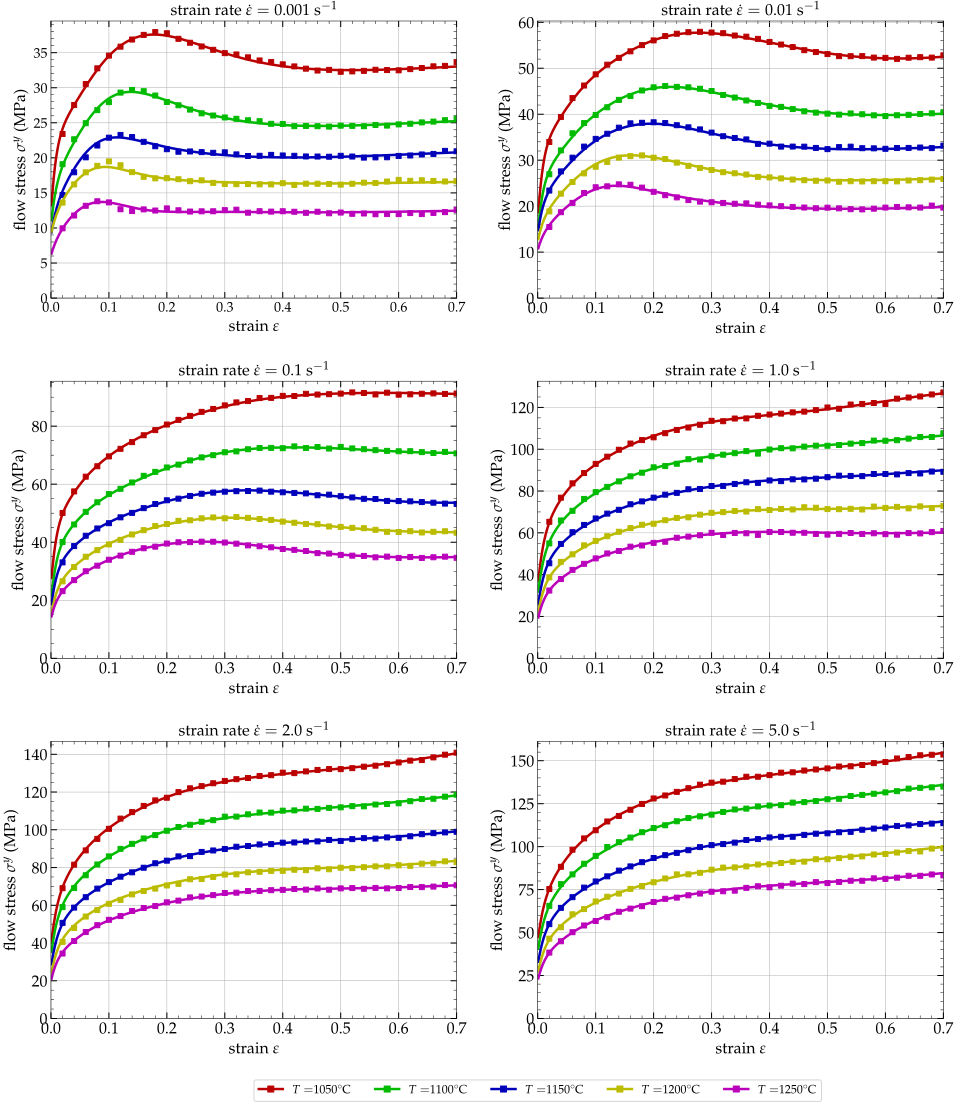
\includegraphics[width=\columnwidth]
{Figures/CompExp-3-15-7-1-sigmoid}
\caption{Comparison between the experimental flow stresses and those predicted by the the 3-15-7-1-sigmoid ANN model}
\label{fig:CompExp-3-15-7-1-sigmoid}
\end{figure}
The experimental data and the ANN prediction correlate very well over the entire range of data and the predicted data can track the hardening and softening regions of the hot deformed material well.
For the ANN model, $\AARE=0.62~\%$ and $\RMSE=0.38~\MPa$ which is excellent.
This model can be used to simulate the hot deformation of this type of alloy with much greater fidelity to the actual material behavior than the analytical models presented previously.

%----------------------------------------------------------------------------------
\subsection{Comparison of analytical and ANN models\label{sec:Comparison}}
%----------------------------------------------------------------------------------

A summary of the coefficients for evaluating the high-temperature flow stress prediction capability of the medium carbon alloy for all models presented in this work is reported in Table \ref{tab:Errors}.
\begin{table}[h!]
\centering
\caption{Accuracy coefficients for all the analyzed models.}
\begin{tabular}{lcccccc}
	\hline
	Coefficients        &   JC    &   MZA   &   HS   &   AR   &  PTM   &  ANN   \\ \hline
	$\AARE(\%)$         & $14.05$ & $21.20$ & $7.75$ & $3.56$ & $4.79$ & $0.62$ \\
	$\RMSE(\MPa)$ & $12.00$ & $19.57$ & $3.80$ & $2.18$ & $4.59$ & $0.38$ \\ \hline
\end{tabular}
\label{tab:Errors}
\end{table}
From this table, we can see that the ANN model has a much better predictive capacity than all the analytical models presented previously. Globally, the values of $\AARE$ and $\RMSE$ are $6$ times lower than with the best of the analytical models, \ie, the Arrhenius model, quoted as reference in the context of the hot forming of alloys \cite{Liang-2022}.

The ANN, Arrhenius and PTM models are the only models that take into account softening with the deformation of medium carbon at low strain rate, unlike the other three models, which only present an increase in the flow stress with the strain, irrespective of the strain rate and temperature, hence their poor performance in predicting the behavior of this material and more particularly at low strain rates.
The parameters reported in Table \ref{tab:Errors}, the correlations that can be seen in Figures \ref{fig:CompExp-JC-6} to \ref{fig:CompExp-3-15-7-1-sigmoid} allow to conclude  that the ANN model is the most efficient of all the models presented when it comes to describing the behavior of the medium carbon alloy for high temperature deformation applications.

%----------------------------------------------------------------------------------
\section{Interpolation and Extrapolation Capability of Analytical and ANN Models \label{sec:IntExt}}
%----------------------------------------------------------------------------------

In order to better compare the performances of the models presented previously (the 5 analytical models and the neural network based model), in this section, we present the ability of each of these models to interpolate and extrapolate the results as a function of the strain rate $\mdot\varepsilon$.
The identification of the performed models is based on a set of experimental data corresponding to 6 strain rates, 5 temperatures and strains ranging from $0$ to $0.7$. To test the learning capacity and fidelity of these models, we propose here to perform the training of the models on only 5 strain rates by voluntarily omitting the strain rate $\mdot\varepsilon=1~\ps$ or $\mdot\varepsilon=5~\ps$.

Thus, one of the omitted strain rates ($\mdot\varepsilon=1~\ps$) is within the range of strain rates for model identification ($0.001~\ps\text{ to }5~\ps$), and therefore, we can test the ability of the models to interpolate the results from the other 5 strain rates and be able to quantify any deviation from experimental values.
On the other hand, since the omitted strain rate ($\mdot\varepsilon=5~\ps$) is outside the range of strain rates for the model identification ($0.001~\ps\text{ to }2~\ps$), we will test the ability of the models to extrapolate results and quantify deviation with the experimental values.

%----------------------------------------------------------------------------------
\subsection{Interpolation validation}
%----------------------------------------------------------------------------------

For the interpolation validation, the chosen omitted strain rate is $\mdot\varepsilon=1~\ps$ and those used for identification (or training for ANN) are the 5 others, \ie $\mdot\varepsilon=[0.001, 0.01, 0.1, 2, 5]~\ps$. All models were re-identified from the same experimental data on a data set corresponding to 5 strain rates and 5 temperatures.

Figure \ref{fig:CompInt} shows a comparison, for strain rate $\mdot\varepsilon=1~\ps$, of the flow stresses $\sigma^y$ calculated by the models (as a line) and the experimental results (as points) for the 5 analytical models and the neural network.
\begin{figure}[!ht]
\centering
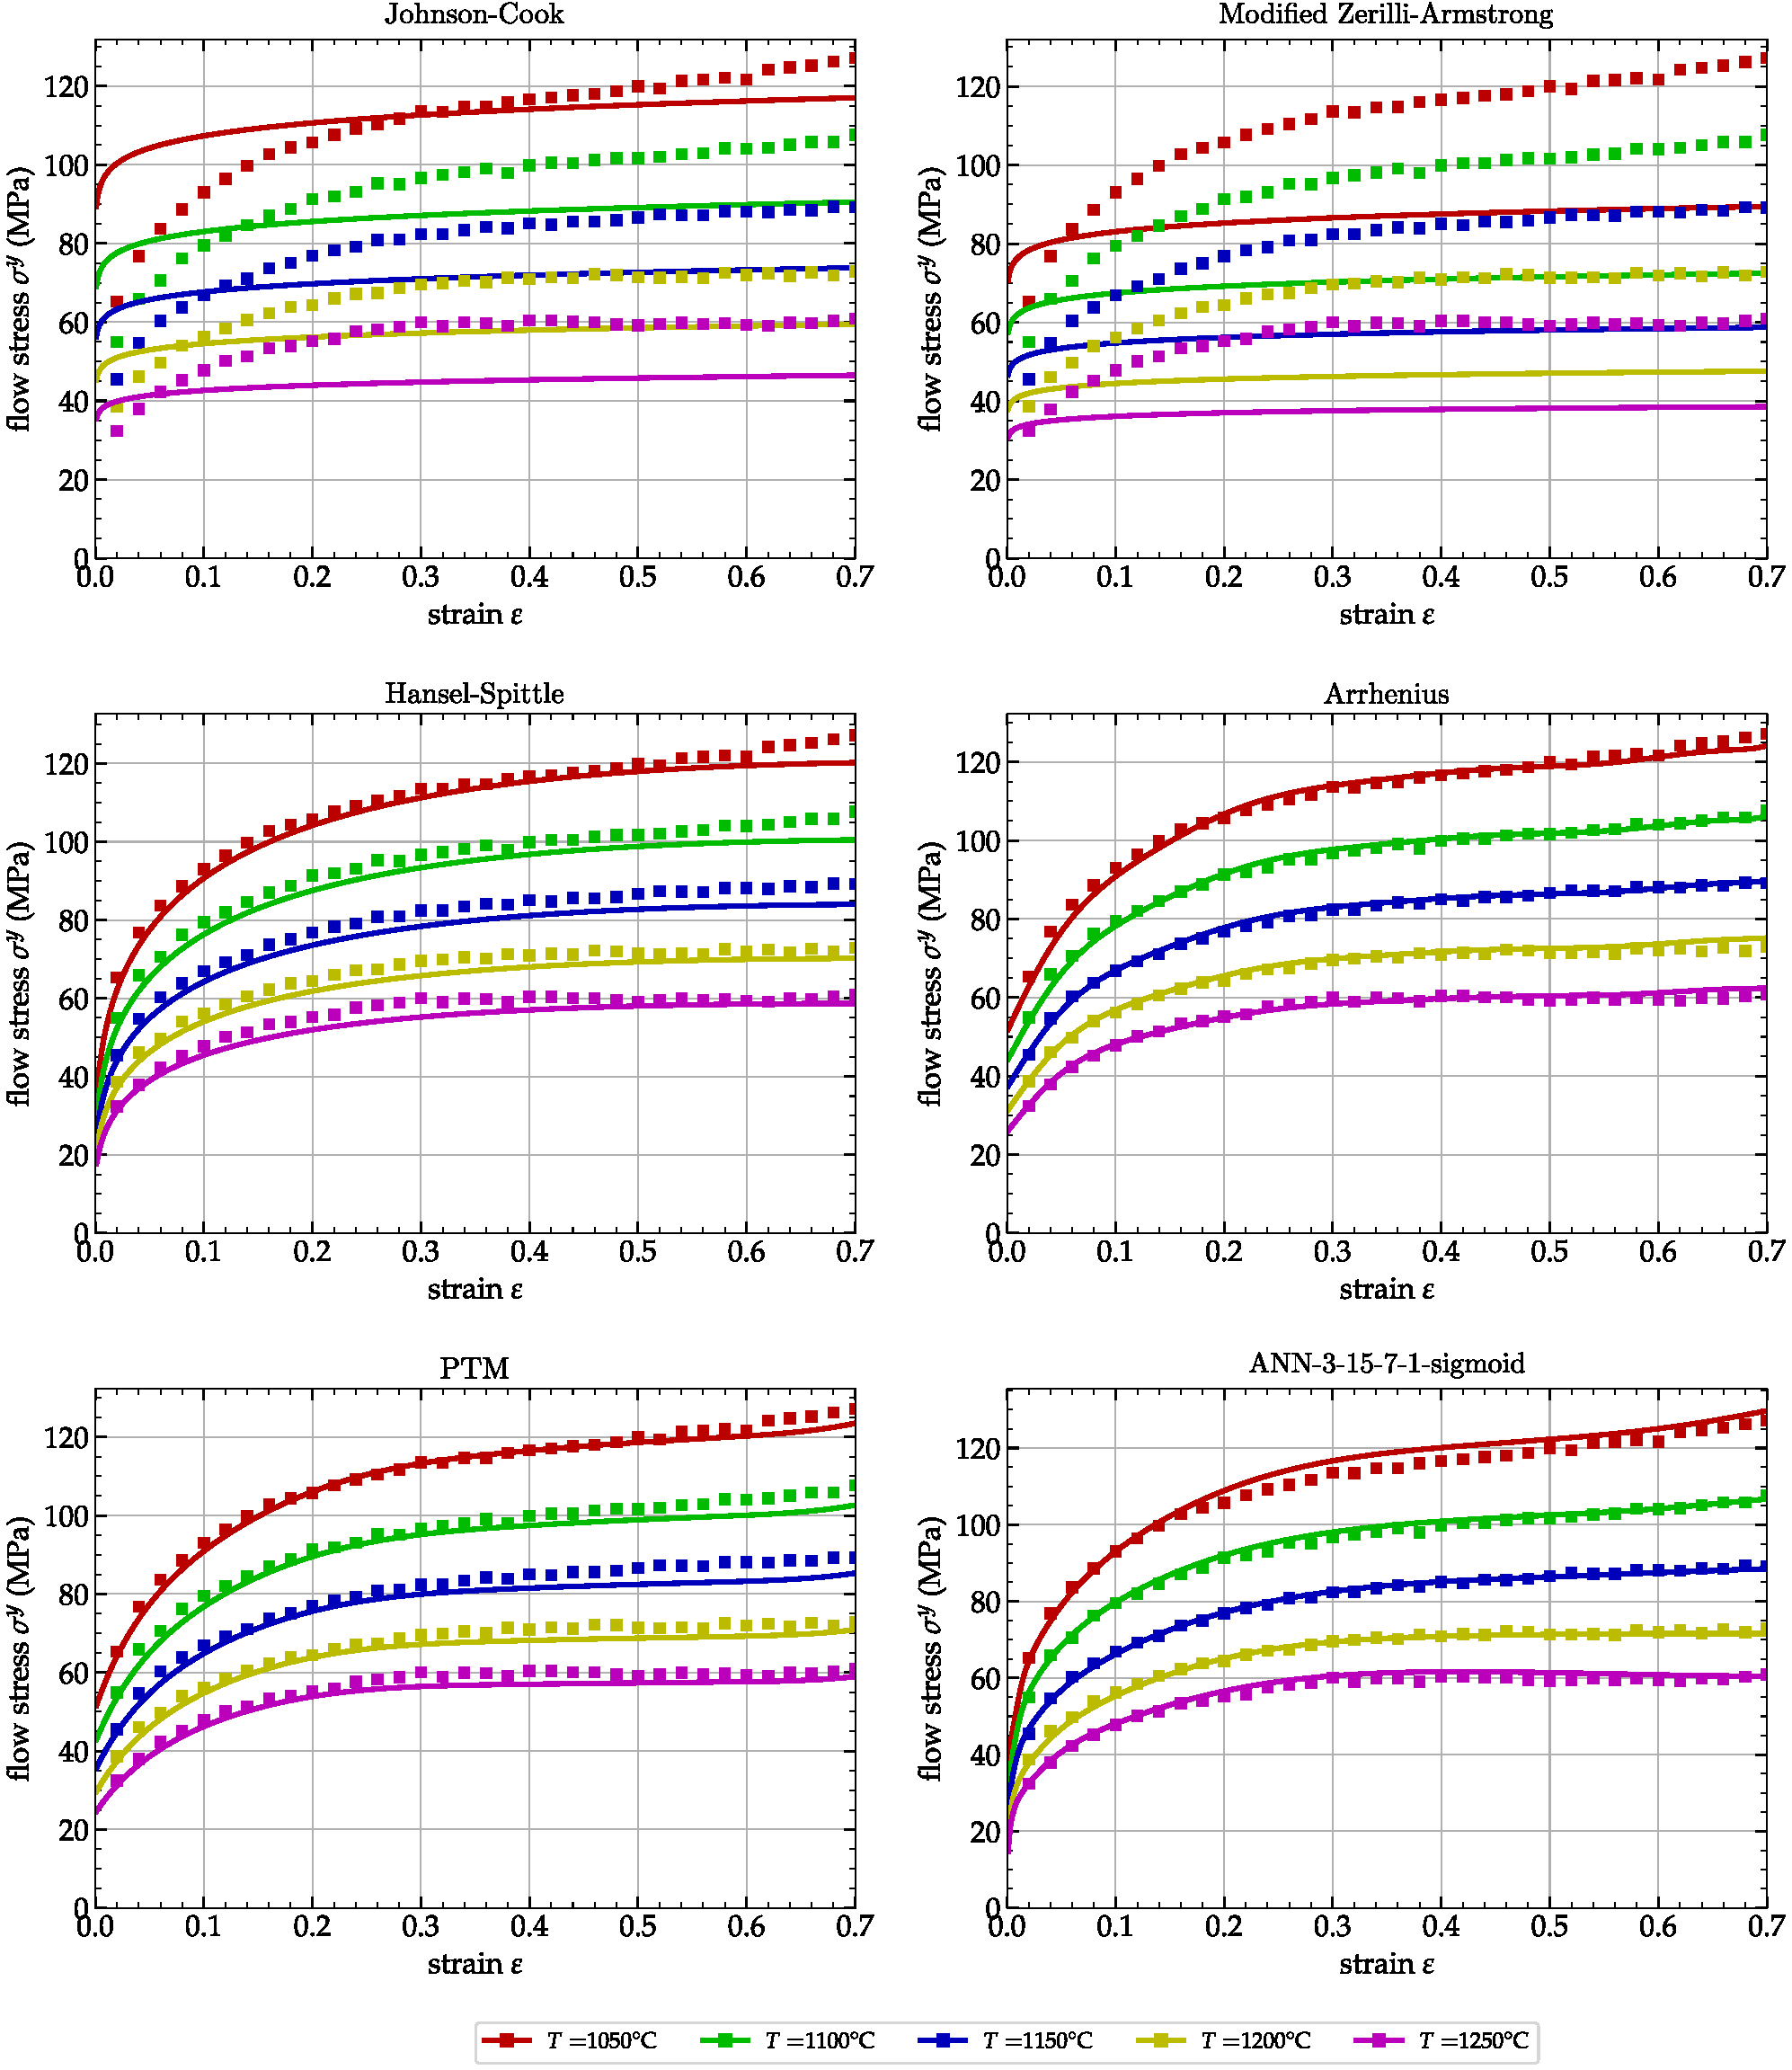
\includegraphics[width=\columnwidth]
{Figures/CompInt}
\caption{Comparison between the experimental (dot) and predicted flow stresses $\sigma^y$ (lines) for $\mdot\varepsilon=1~\ps$}
\label{fig:CompInt}
\end{figure}
Table \ref{tab:IntVal} shows the $\AARE$ and $\RMSE$ deviations between the different models and the experimental data calculated either for the 6 strain rates (lines referred as: all) or only on the strain rate $\mdot\varepsilon=1~\ps$.
\begin{table}[h!]
\centering{}
\caption{Accuracy coefficients of interpolation for all models with  $\mdot\varepsilon=1~\ps$}
\begin{tabular}{llcccccc}
	\hline
	Strain rate                      & Coefficients        &   JC    &   MZA   &   HS   &   AR   &  PTM   &  ANN   \\ \hline
	\mr{2}{id. $\mdot\varepsilon$}   & $\AARE(\%)$         & $13.79$ & $20.22$ & $8.57$ & $3.96$ & $5.10$ & $0.70$ \\
	                                 & $\RMSE(\MPa)$ & $11.83$ & $19.00$ & $3.97$ & $2.29$ & $4.73$ & $0.38$ \\ \hline
	\mr{2}{$\mdot\varepsilon=1~\ps$} & $\AARE(\%)$         & $14.87$ & $27.79$ & $3.74$ & $1.46$ & $3.16$ & $2.47$ \\
	                                 & $\RMSE(\MPa)$ & $12.02$ & $23.67$ & $3.10$ & $1.46$ & $2.65$ & $2.77$ \\ \hline
	\mr{2}{all $\mdot\varepsilon$}   & $\AARE(\%)$         & $14.42$ & $28.90$ & $7.55$ & $3.45$ & $4.90$ & $0.96$ \\
	                                 & $\RMSE(\MPa)$ & $11.86$ & $19.86$ & $3.84$ & $2.17$ & $4.45$ & $1.18$ \\ \hline
\end{tabular}
\label{tab:IntVal}
\end{table}

In Figure \ref{fig:CompInt} it can be seen that the first two models (JC and MZA), presented in this study do not have the ability to reproduce the behavior of the material for the strain rate $\mdot\varepsilon=1~\ps$.
Overall, the JC model gives better results than the MZA model for $\mdot\varepsilon=1~\ps$, which is reflected in Table \ref{tab:IntVal} by a lower value of $\AARE$ and $\RMSE$ for JC than for MZA.
Nevertheless, these values are higher than $10\%$ for the JC model and $20\%$ for the MZA model, which reflects the poor ability of these models to correctly model the behavior of this material.
This finding is in agreement with the previous findings of Sections \ref{sec:JC} and \ref{sec:MZA} which showed the inability of these models to take into account the softening of the behavior visible at low strain rates and low temperatures.

From a general appearance point of view, the other 4 models, HS, AR, PTM and ANN, give globally similar results with a higher fidelity for the AR and ANN models compared to the other two models.
Table \ref{tab:IntVal} shows a quantitative comparison on $\AARE$ and $\RMSE$ for three different cases: on the 5 identified strain rates (named id. $\mdot\varepsilon$), on only the strain rate $\mdot\varepsilon=1~\ps$ and on all 6 strain rates for these 6 models.
It appears from this Table that while the two models, AR and ANN, give equivalent (and excellent) results concerning the values of $\AARE$ and $\RMSE$ for the strain rate $\mdot\varepsilon=1~\ps$, the ANN model gives a globally better result across the entire strain rates spectrum, with values of $\AARE=0.96\%$ and $\RMSE=1.18~\MPa$ respectively, that is to say, values approximately 2 to 3 times lower for the ANN model than for the AR model.

This shows the superior fidelity of the ANN model compared to the 5 analytical models presented in this study both in the interpolation capability of the model and in the overall behavior.

%----------------------------------------------------------------------------------
\subsection{Extrapolation validation}
%----------------------------------------------------------------------------------

For validation of the models' ability to extrapolate, the omitted strain rate chosen is $\mdot\varepsilon=5~\ps$ and those used for identification are $\mdot\varepsilon=[0.001, 0.01, 0.1, 1, 2]~\ps$.
The strain rate omitted in this analysis therefore has the highest value, which restricts the learning domain.

In this new identification configuration, Figure \ref{fig:CompExt} shows a comparison, for strain rate $\mdot\varepsilon=5~\ps$, of the flow stresses $\sigma^y$ computed by the models (as a line) and the experimental results (as points) for the 5 analytical models and the neural network.
\begin{figure}[!ht]
\centering
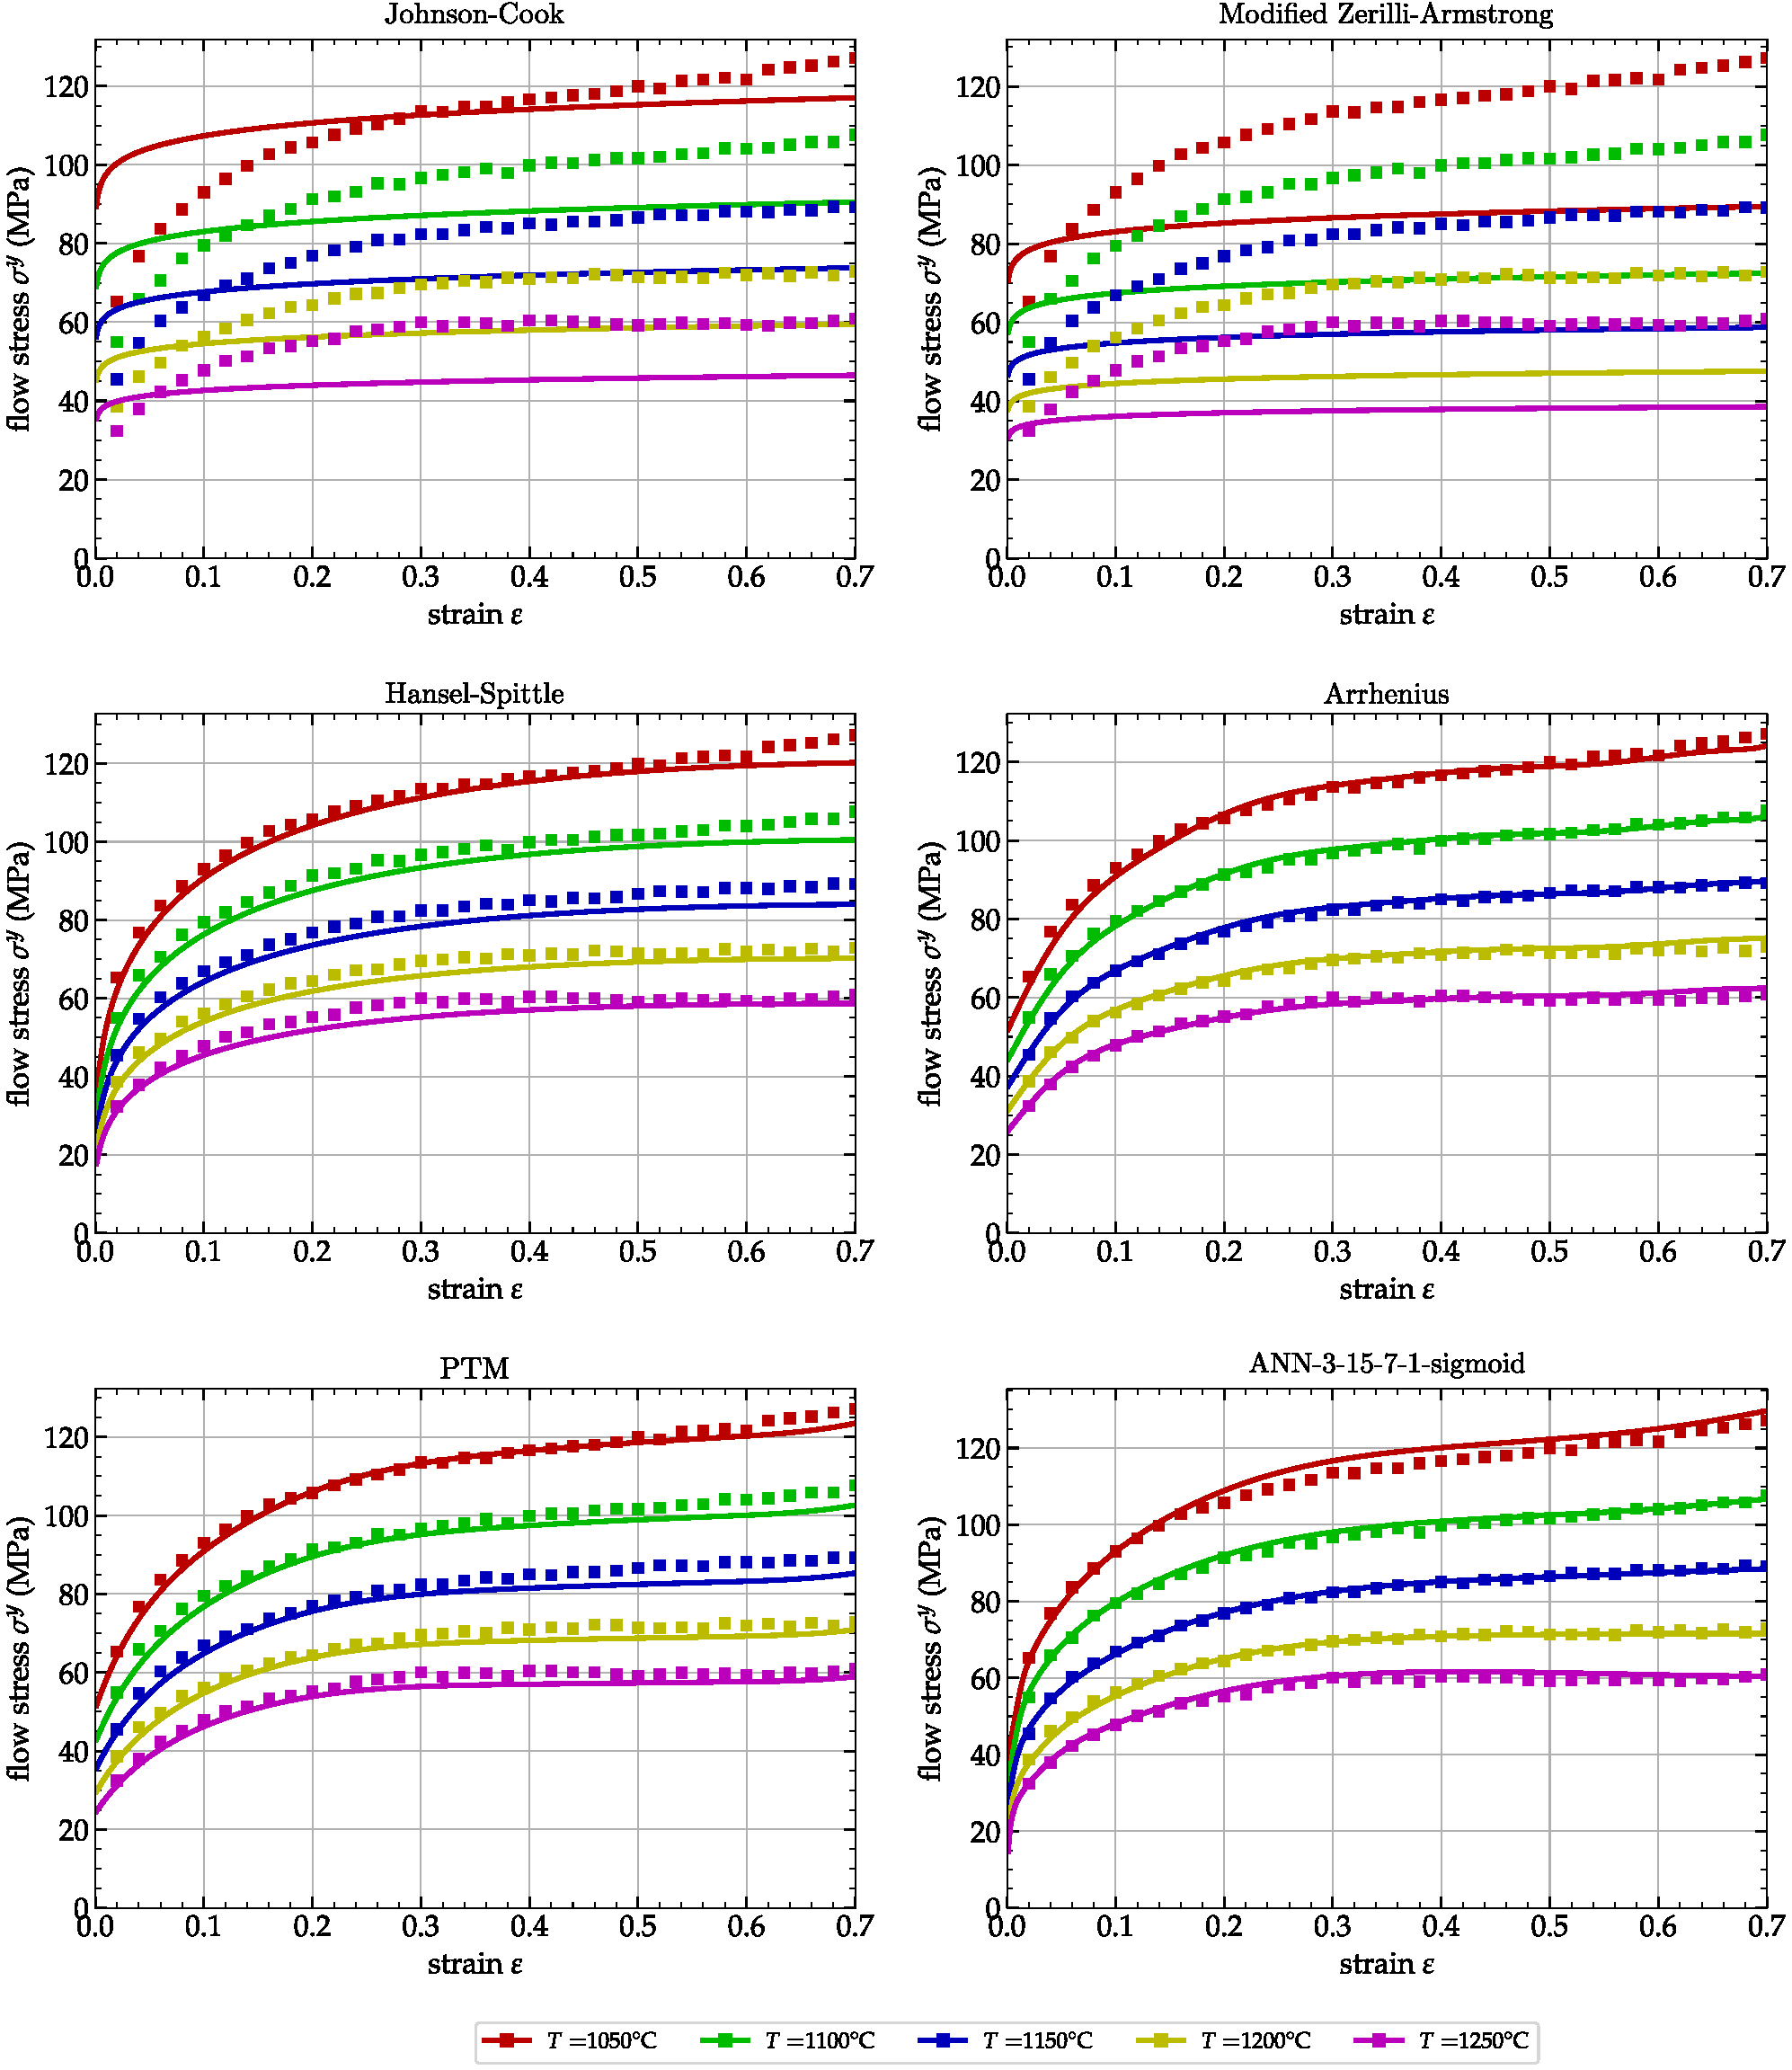
\includegraphics[width=\columnwidth]
{Figures/CompExt}
\caption{Comparison between the experimental (dot) and predicted flow stresses $\sigma^y$ (lines) for $\mdot\varepsilon=5~\ps$}
\label{fig:CompExt}
\end{figure}
Table \ref{tab:ExtVal} shows the $\AARE$ and $\RMSE$ deviations between the different models and the experimental data calculated either for the 6 strain rates (lines referred as: all) or only on the strain rate $\mdot\varepsilon=5~\ps$.
\begin{table}[h!]
\centering{}
\caption{Accuracy coefficients of extrapolation for all models with  $\mdot\varepsilon=5~\ps$}
\begin{tabular}{llcccccc}
	\hline
	Strain rate                      & Coefficients        &   JC    &   MZA   &   HS   &   AR   &   PTM   &  ANN   \\ \hline
	\mr{2}{id. $\mdot\varepsilon$}   & $\AARE(\%)$         & $13.09$ & $19.09$ & $7.30$ & $4.03$ & $4.34$  & $0.61$ \\
	                                 & $\RMSE(\MPa)$ & $9.86$  & $16.26$ & $3.36$ & $2.32$ & $3.63$  & $0.32$ \\ \hline
	\mr{2}{$\mdot\varepsilon=5~\ps$} & $\AARE(\%)$         & $20.16$ & $24.27$ & $7.73$ & $3.53$ & $11.46$ & $3.87$ \\
	                                 & $\RMSE(\MPa)$ & $20.73$ & $25.95$ & $7.83$ & $4.02$ & $12.91$ & $5.84$ \\ \hline
	\mr{2}{all $\mdot\varepsilon$}   & $\AARE(\%)$         & $15.12$ & $25.87$ & $7.12$ & $3.86$ & $5.34$  & $1.09$ \\
	                                 & $\RMSE(\MPa)$ & $12.36$ & $18.24$ & $4.43$ & $2.68$ & $6.23$  & $2.40$ \\ \hline
\end{tabular}
\label{tab:ExtVal}
\end{table}

As presented in the previous section regarding the interpolation capability of the models, in Figure \ref{fig:CompExt} it can be seen that the first two models, JC and MZA, in this study again do not have the ability to correctly reproduce the material behavior for the strain rate $\mdot\varepsilon=5~\ps$.
The JC model performs better than the MZA model for $\mdot\varepsilon=5~\ps$, which is reflected in Table \ref{tab:ExtVal} by a lower value of $\AARE$ and $\RMSE$ for JC than for MZA.
Nevertheless, these values are too large for proper use.
Once again, it is the inability of these models to take into account the softening of the behavior at low strain rates and low temperatures that is at the origin of these values.

The other 4 models, HS, AR, PTM and ANN, give better results with higher fidelity for the AR and ANN models than for the other two models.
Table \ref{tab:ExtVal} shows a comparison over all strain rates and over $\mdot\varepsilon=5~\ps$ for these 6 models.
The HS model performs worse on extrapolation than the AR and ANN models, while the PTM model is relegated to the last position in this ranking with values of $\AARE$ and $\RMSE$ greater than $10\%$ for the strain rate $\mdot\varepsilon=5~\ps$.
The two models, AR and ANN, give the best results for the values of $\AARE$ and $\RMSE$ for the strain rate $\mdot\varepsilon=5~\ps$.
Tis time, the AR model performs a little better on the $\mdot\varepsilon=5~\ps$ strain rate as compared to the ANN model, but the latter gives  a globally better result across the entire strain rates spectrum, with values of  $\AARE=1.09\%$ and $\RMSE=2.40~\MPa$ respectively.

We can therefore conclude from this part of the study that the AR model is the best performing of the 5 analytical models presented, which is in agreement with the fact that it is widely used for thermomechanical processing, but the ANN model approach has advantages over the AR model approach in that, overall, the ANN model is more faithful to experimental data than is the AR model, for all strain rates.

%----------------------------------------------------------------------------------
\subsection{Proposed technique for better interpolation}
%----------------------------------------------------------------------------------
\begin{figure}[!ht]
\centering
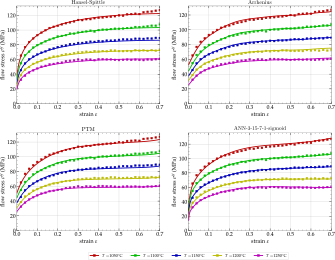
\includegraphics[width=\columnwidth]
{Figures/Performance}
\caption{Comparison between experimental (dot) and predicted flow stresses $\sigma^y$ (lines) for $\mdot\varepsilon=1~\ps$}
\label{fig:Performance}
\end{figure}
In this section a technique is proposed to obtain a better interpolation of data. Indeed, as mentioned in the introduction, it is important to know how to ensure the effectiveness of the model that well describes the behavior of a material for a good use on new data different from those used for its identification. It is therefore a question of choosing models that have a good correlation with experience and proposing a formula for a good use of their parameters on unknown data. The AR, HS, PTM and ANN models are therefore chosen and it emerges that each model must be multiplied by a lambda factor whose formula is given as follows.
\begin{equation}
 \lambda = \left(\frac{\dot{\varepsilon}_{max} - \dot{\varepsilon}_{p} }{\dot{\varepsilon}_{p} - \dot{\varepsilon}_{min}}\right)^{\frac{\dot{\varepsilon}_p}{m}}
\end{equation}
Where $\dot{\varepsilon}_{p}$ is the unknown strain rate and $m\in[50-300]$
Applying this formula, the new figures are plotted in Figure \ref{fig:Performance}. These results are clearly better than the initial ones. 

\section{Conclusions and future work\label{sec:Conclusion}}
%----------------------------------------------------------------------------------

Experimental tests were performed on a Gleeble thermomechanical simulator for a modified medium carbon alloy to investigate the applicability and predictive accuracy of 5 analytical models and an Artificial Neural Network model over a range of strains ($0.0-0.7$), strain rates ($0.001~\ps-5~\ps$) and temperatures ($1050\celsius-1250\celsius$).
The analytical models selected for this study were the Johnson-Cook (JC) model \cite{Johnson-1983}, the Modified Zerilli-Armstrong (MZA) model \cite{Samantaray-2009}, the Hansel-Spittle (HS) model \cite{Hensel-1978}, the Arrhenius (AR) model \cite{Sellars-1966} and the PTM model  \cite{TizeMha-2022}.
An analysis of the data from the Gleeble trials, and comparison of the 6 models proposed in this study against the experiments, led to the following conclusions.

From an experimental point of view, it appears from the tests carried out that the flow stress $\sigma^y$ increases with a decrease of the temperature $T$ and an increase of the strain rate $\mdot\varepsilon$ due to the competitive appearance of the dynamic softening and work hardening mechanisms.
The dynamic recrystallization (DRX) phenomenon, introduced through the difference between the maximum and permanent strain, shows a partially complete microstructure evolution.
Thus, at high strain rates, it is difficult to visualize the DRX phenomenon on the flow curves due to the sensitivity of this phenomenon to the strain rate.
A study focused on an in-depth analysis of the microstructure of this steel alloy and its impact on mechanical properties is currently underway.

Five analytical models and an Artificial Neural Network-based model were identified for this alloy,
Among the analytical models, the JC and MZA models proved inadequate to reproduce the behavior of this material, while the HS, PTM and AR models showed their capabilities, presenting an acceptable $\AARE$ error (from $3.5\%$ to $7.7\%$). The AR model (with a $3.56\%$ error) proved superior to the other two, thus justifying its use in thermomechanical processes. The ANN model, is largely more accurate than the analytical models in predicting the flow stress $\sigma^y$ of the medium carbon with a $\AARE=0.62\%$.

To test the performance of each proposed model, a study was conducted to evaluate the interpolation and extrapolation capability of the developed models.
In the case of interpolation, the HS, PTM and AR models correlated well with the experiment, but the ANN model was superior, with an error factor 5 times lower than the AR model.
For data extrapolation, the HS, PTM and AR models again correlated well with the experiment, but the ANN model once again performed better globally. These two parts of the study confirm what was demonstrated in the model identifications.

Identifying the parameters of an ANN model from experimental data requires more time than identifying the parameters of analytical models (about 40 minutes on a working laptop), but as shown by Pantalé \eal \cite{Pantale-2021}, implementing an ANN model in a computational code is straightforward.
Therefore, we recommend using the ANN model when conducting a study involving this alloy under the experimental conditions examined here in.

For future work perspectives, we will develop another ANN model to characterize the microstructure in terms of DRX and the formation of phases such as ferrite, bainite and martensite for example.
This ANN model can then be compared to the most commonly used classical models such as the JMAK model.
Then, these ANN models will be implemented in FEM software such as Abaqus or Forge in order to validate them.

\bibliographystyle{elsarticle-num}
\bibliography{Bibliography}

%----------------------------------------------------------------------------------
\section*{Appendix\label{sec:Appendix}}
%----------------------------------------------------------------------------------

In order to complete this paper, we report here after the computing process and the $180$ coefficients of the Artificial Neural Network ANN-3-15-7-1-sigmoid model used in Section \ref{sec:ANNmodel}.
In order to use this model we describe $\sigma^y$ from the input variables $\varepsilon^p$, $\mdot\varepsilon$ and $T$ after the procedure to compute the flow stress. This process can be decomposed into 3 phases:
\begin{itemize}
\item We first have to normalize the input values of the ANN $x_i$ within the range $[0,1]$ to avoid an ill-conditioned system as presented by many other authors in the literature \cite{Lin-2008-ANN, Lu-2011-ANN}.
Therefore, the three components of the input vector $\overrightarrow{x}$ are obtained from the plastic strain $\varepsilon^p$, the plastic strain rate $\mdot{\varepsilon}^p$ and the temperature $T$ using the following expressions:
\begin{equation}
\overrightarrow{x}=
\begin{cases}
x_1 = \frac{\varepsilon^p - [\varepsilon^p]_{min}}{[\varepsilon^p]_{max} - [\varepsilon^p]_{min}}\\
x_2 = \frac{\ln(\mdot{\varepsilon}/\mdot{\varepsilon_0})-[\ln(\mdot{\varepsilon}/\mdot{\varepsilon_0})]_{min}}{[\ln(\mdot{\varepsilon}/\mdot{\varepsilon_0})]_{max}-[\ln(\mdot{\varepsilon}/\mdot{\varepsilon_0})]_{min}}\label{eq:CR1}\\
x_3 = \frac{T-[T]_{min}}{[T]_{max}-[T]_{min}}
\end{cases}
\end{equation}
where $[~]_{min}$ and $[~]_{max}$  are the boundaries of the range of the corresponding field: $\varepsilon^p\!\in\!\left[0.0,0.7\right]$, $\mdot{\varepsilon}\!\in\!\left[0.001~\ps,5.0~\ps\right]$, $T\!\in\!\left[1050~\celsius,1250~\celsius\right]$ and $\sigma\!\in\!\left[1.311~\MPa,153.739~\MPa\right]$.
The reference strain rate is $\mdot{\varepsilon_0} = 0.001~\ps$.
\item Then we compute the output $s$ of the ANN from the input vector $\overrightarrow{x}$ using the  following three equations.
\begin{equation}
\overrightarrow{y}_1 = \left[1 + \exp{\left(- \w_1 \dotp \overrightarrow{x}- \overrightarrow{b}_1\right)}\right]^{-1}
\end{equation}
\begin{equation}
\overrightarrow{y}_2 = \left[1 + \exp{\left(- \w_2 \dotp \overrightarrow{y}_1- \overrightarrow{b}_2\right)}\right]^{-1}
\end{equation}
\begin{equation}
s = \overrightarrow{w}^T \dotp \overrightarrow{y}_2 + b
\end{equation}
\item Finally, the flow stress $\sigma^y$ can be obtained from the output $s$ of the ANN using the following equation:
\begin{equation}
\sigma^y =  \left([\sigma]_{max}-[\sigma]_{min}\right)s + [\sigma]_{min} \label{eq:CR2}
\end{equation}
\end{itemize}

Conforming to the computing process proposed by Equations (\ref{eq:CR1}-\ref{eq:CR2}), we report hereafter the $180$ coefficients of the ANN-3-15-7-1-sigmoid model used in Section \ref{sec:ANNmodel}.
The weight matrix for the first hidden layer $\w_1$ is a $15\times3$ matrix:
\begin{equation*}
\w_1 = \left[
\begin{array}{rrr}
2.2206 & -3.7555 & -6.7246\\
-4.8598 & 5.7431 & -5.8538\\
2.3099 & 3.3325 & -5.1795\\
2.0475 & 0.8006 & -1.4259\\
8.8358 & -6.0362 & 0.8226\\
-1.2613 & -0.9274 & -2.3725\\
-0.3561 & 6.5032 & -10.7573\\
-11.7226 & -2.0455 & 1.2248\\
3.1066 & 26.5580 & 18.6540\\
-0.5150 & -5.6922 & 1.0104\\
-6.4755 & 8.4888 & -2.4459\\
-1.8791 & -0.5380 & 2.2295\\
-6.0206 & 1.2776 & 0.2169\\
0.2619 & -4.7974 & -1.1282\\
-27.1456 & -0.5327 & -0.5303\\
\end{array}\right]
\end{equation*}
The bias of the first hidden layer $\overrightarrow{b_1}$ is a $15$ components vector:
\begin{equation*}
\overrightarrow{b}_1 = \left[
\begin{array}{r}
5.9164\\
-1.9074\\
-2.6837\\
-1.0954\\
-0.9509\\
3.1682\\
-4.3964\\
0.6343\\
-5.0676\\
2.0228\\
1.1267\\
-0.9671\\
-0.6263\\
2.3110\\
-0.3037\\
\end{array}\right]
\end{equation*}
The weight matrix for the second hidden layer $\w_2$ is a $7\times15$ matrix:
\begin{equation*}
\w_2^T = \left[
\begin{array}{rrrrrrr}
-0.5783 & 1.2724 & 0.5747 & 0.6449 & -4.2203 & -0.2380 & 0.2591\\
-0.4852 & 5.2807 & 0.8888 & -8.2324 & -2.0075 & -0.6474 & -1.0787\\
4.4499 & -0.0137 & 0.1657 & 0.3198 & 4.9765 & -1.2503 & 0.8219\\
1.7571 & 0.7730 & 0.0208 & -1.3316 & -0.8945 & -0.7284 & -0.1831\\
-1.0866 & 0.1330 & -0.8615 & -0.1283 & 0.2218 & -0.1772 & -2.7458\\
-0.3925 & 1.3994 & 0.0630 & -1.8397 & -1.1047 & -1.9839 & 0.5767\\
-0.2121 & 0.9977 & 1.2028 & -9.6525 & 0.5520 & 0.1062 & -0.0409\\
-1.1518 & -1.6402 & -4.1501 & -1.0759 & 0.4749 & -2.8350 & 0.9225\\
-1.1453 & -0.2173 & -0.1382 & 0.8264 & -0.5125 & 0.1882 & -0.8654\\
-4.3301 & -0.3711 & -7.4305 & 3.5926 & -9.6217 & -1.2375 & 1.6171\\
2.3907 & -1.0085 & -0.8828 & -1.1891 & 0.9947 & 1.1178 & -1.0953\\
-1.5955 & 1.6313 & 0.4916 & 0.1906 & -1.9216 & -1.4140 & 1.3827\\
-1.6985 & 1.4277 & -3.4462 & -8.3777 & -1.2132 & -1.2158 & 2.8512\\
-1.9954 & -2.0159 & -8.3455 & -0.5205 & 0.2942 & -1.3337 & 0.2026\\
4.3040 & -0.7164 & -1.0859 & 3.4294 & -23.8003 & 12.5859 & 7.3721\\
\end{array}\right]
\end{equation*}
The bias of the second hidden layer $\overrightarrow{b_2}$ is a 7 component vector:
\begin{equation*}
\overrightarrow{b}_2 = \left[
\begin{array}{r}
0.7534\\
0.9473\\
0.6055\\
-0.7793\\
-1.0305\\
-1.5779\\
-0.1471\\
\end{array}\right]
\end{equation*}
The weight vector for the output layer $\overrightarrow{w}$ is a 7 component vector:
\begin{equation*}
\overrightarrow{w} = \left[
\begin{array}{r}
0.1920\\
0.3406\\
0.3839\\
-0.2880\\
1.2047\\
-1.4126\\
-0.2215\\
\end{array}\right]
\end{equation*}
The bias of the output layer $b$ is a scalar:
\begin{equation*}
b = 0.1178
\end{equation*}

\end{document}